\documentclass[
12pt,
a4paper,
twoside
% fullpage 
]{report}
\usepackage{graphics}
\usepackage{epsf,graphicx}%, amstext,url} 
\usepackage{pdfpages}
\usepackage{amsmath}
\usepackage{todonotes}
\usepackage{listings}
\usepackage{braket}
\usepackage{cancel}
\usepackage{url}
\usepackage[version=4]{mhchem}
\bibliographystyle{unsrt}
\usepackage{lipsum}
\setlipsum{%
  par-before = \begingroup\color{lightgray},
  par-after = \endgroup
}
% \usepackage[top=2cm,bottom=4cm,left=1.5cm,right=3cm,asymmetric]{geometry}
\usepackage[a4paper,width=155mm,top=25mm,bottom=25mm]{geometry}
\newcommand{\td}[1]{\todo[]{#1}}
\newcommand{\tdr}[1]{\todo[color=red]{#1}}
\newcommand{\tdg}[1]{\todo[color=green]{#1}}

\usepackage{setspace}
\doublespacing
\usepackage{imakeidx}
% \makeindex
\makeindex[columns=2, title=Index of Terms, intoc]

% \usepackage{hyperref}

\RequirePackage[hidelinks]{hyperref} % 

\begin{document}
\thispagestyle{empty}

%
%	This is a basic LaTeX Template for the TP/MP MSc Dissertation report

\parindent=0pt          %  Switch off indent of paragraphs 
\parskip=5pt            %  Put 5pt between each paragraph  

% \documentclass[
12pt,
a4paper,
% fullpage 
]{report}
\usepackage{graphics}
\usepackage{epsf,graphicx}%, amstext,url} 
\usepackage{afterpage}
\begin{document}
%	This section generates a title page
%       Edit only the sections indicated to put in the project title, and submission date
\begin{titlepage}
\vspace*{0.1\textheight}

\begin{center}
        \huge{\bfseries Title of my Dissertation}\\ % Replace with the title of your dissertation!
\end{center}

\medskip

\begin{center}
        \Large{Conner J Adlington}\\  % Author of dissertation - replace with your name!
        \medskip
        \large{August XX, 2024}  % Submission date
\end{center}

%%% If necessary, reduce the number 0.4 below so the University Crest
%%% and the words below it fit on the page.
%%% Don't let the crest, or the wording below it, flow onto the next page!

\vspace*{0.3\textheight}

\begin{center}
        
\includegraphics[width=35mm]{../crest.pdf}
\end{center}

\medskip

\begin{center}

%%%
%%% Change Theoretical to Mathematical if appropriate
%%%
\large{
  MSc in Theoretical Physics\\[0.8ex]
  The University of Edinburgh\\[0.8ex]
  2023}

\end{center}

\end{titlepage}

\end{document}


\includepdf[pages=-]{Title/title.pdf}

\pagenumbering{roman}

\begin{abstract}
	\topskip0pt
\vspace*{\fill}
\begin{center}
\textrm{\bfseries\Huge Abstract}%
\end{center}%
    % the context or background information for your research; the general topic under study; the specific topic of your research
Spin based sensing, particularly with silicon carbide is a growing and exciting field. A great deal of work has gone into developing complex sensing regimes to enable the detection of the magnetic and electric fields, strain, pressure and temperature with nanoscale sensors. 
    % the central questions or statement of the problem your research addresses
This work provides a detailed overview of how that sensing is achieved across both $S=1$ and $S=3/2$ systems, particularly with reference to colour centres in Silicon Carbide. 
    % what’s already known about this question, what previous research has done or shown
Whilst sensing in one mode i.e. detecting one parameter in isolation is well understood, borrowing a lot from the work done with the Diamond Nitrogen vacancy, there is not a great deal of work on where these devices may be used to simultaneously measure multiple parameters. 
    % the main reason(s), the exigency, the rationale, the goals for your research—Why is it important to address these questions? Are you, for example, examining a new topic? Why is that topic worth examining? Are you filling a gap in previous research? Applying new methods to take a fresh look at existing ideas or data? Resolving a dispute within the literature in your field? . . .
Multimodal sensors could have applications ranging from the laboratory to space and life sciences. We first provide a detailed account of methods already used for single mode sensing. Each schema is given a clear summary which describes the limitations of its implementation. We then attempt to combine the schemas to see which are compatible.
%
    % your research and/or analytical methods
    % your main findings, results, or arguments
We propose four possible combinations of modes and suggest how future work may resolve at least two more combinations. This research thus allows for the implementation of the multimodal techniques by combining existing techniques and may help to direct future research to further develop the field of multimodal sensing. 
    % the significance or implications of your findings or arguments.
\vspace{1em}
% \todo[inline, color=red]{Need to write an abstract}
\begin{center}
    {\color{figcaption}\rule{0.75\textwidth}{0.1pt}}
\end{center}
% \newpage

\end{abstract}



\topskip0pt
\vspace*{\fill}
\begin{center}
\textrm{\bfseries\Huge Declaration}%
\end{center}%
\vspace{1em}

I declare that this dissertation was composed entirely by myself. Chapter \ref{ch:background} gives a detailed overview of the science and does not contain original research. Chapter \ref{ch:design} covers the application of the science outlined in the previous chapter and is primarily a collection of already established techniques. For both Chapter \ref{ch:background} and Chapter \ref{ch:design} many of the calculations were made independently and verified by comparison to literature to ensure the consistency of this work. Chapter \ref{ch:results} is entirely my own work and represents the approaches which warranted inclusion in this work. Many more attempts at combining schemas were made, but were unsuccessful and cannot be concisely included in this work. 
Finally, Chapter \ref{ch:conclusions} summarises the work completed, discusses wider scientific context and possible directions for  
future. 

Computer modelling was done using Python where specifically the NumPy, MatPlotLib (Pyplot) and SymPy packages were used to numerically diagonalise and plot Hamiltonians and simulate ODMR spectra. Tikz figures at the start of Chapter \ref{ch:background} are adapted from \url{tikz.net}. All other figures, except where clearly stated, are my own work.  

% \lipsum[1]
% \todo[inline, color=red]{Need to write a declaration}
% Chapters 2 and 3 provide an introduction to the subject area and a
% description of previous work on this topic. They do not contain
% original research.
%
% Chapter~4 describes work that was carried out entirely by me. The results of
% this chapter have been obtained previously by Professor Anne T Matta of the
% University of Kinlochteuchter, but the methods used here are different
% in some important (or minor) ways.
%
% Chapters 4 through 6 contain my original work. The work described in
% Chapter~4 was carried out in collaboration with Professor Carole Ann O'Malley
% and her PhD student Jack O'Bean. Chapter~5 presents original work done
% entirely by me.
%
% \bigskip
%
% State whether calculations were done using Mathematica, Maple, MATLAB,
% SymPy, etc, with (or without) gamma-matrix manipulation code, master
% integrals, the Super-Duper software package, etc. In other words, you
% should refer to any software that you used during your project. For
% example, Monte Carlo simulation packages, hydrodynamics packages,
% measurement code, fitting code, tensor algebra and/or calculus packages,
% Feynman diagram evaluation packages, etc.
%
% State whether any software you used was written by you from scratch,
% by your supervisor (or by whoever), or if it's a standard package.
%
\vspace*{\fill}
\newpage
%
%


\topskip0pt
\vspace*{\fill}
\begin{center}
\textrm{\bfseries\Huge Personal Statement}%
\end{center}%

\vspace{1em}

% \emph{You \textbf{\emph{must}} include a Personal Statement in your
%   dissertation. This should describe what you did during the project,
%   and when you did it. Give an account of problems you faced and how
%   you attempted to overcome them. The examples below are based on
%   personal statements from MSc and MPhys projects in previous years,
%   with (mostly-obvious) changes to make them anonymous. }
%
The project began with developing a deeper understanding of the physics underlying spintronics. 
The focus was on electron paramagnetic resonance (EPR), specifically using the continuous wave optically detected magnetic resonance technique (CW-ODMR). For this, there is a wealth of literature on the diamond nitrogen vacancy (DNV). Most popular is the application of the DNV as a very sensitive magnetometer. 

I worked to  understand the intricacies of the diamond systems, with the intention of applying this knowledge to SiC. 
When I felt comfortable with the underlying physics, I began modelling the different system Hamiltonians. I applied varying $\vec{B}$ and $\vec{E}$ as well as varied temperature. The goal was both to understand the influence of these external factors on the spin-system energy levels as well as to verify my model behaved correctly in the simple cases when compared to existing literature. 

When I had the capability to dynamically model both the DNV and several SiC defects, with different spin numbers, I created ensembles of specifically chosen defects to visualise how the CW-ODMR spectra might change under the influence of varying $\vec{B}$, $\vec{E}$ and $T$. This, as well as existing literature allowed me to isolate specific defects which were most appropriate for the sensing of specific variables. 
For example, the V2 Silicon defect in SiC is very insensitive to changes in temperature so would not be the most appropriate for thermometry application. 

When an ensemble of defects was selected for a specific multi-modal application and the nature of the changes to the ODMR spectra was understood, I worked to develop a method to extract and disentangle the influence of each individual influence on the spectra. 

This process was repeated for several model systems and in the end I developed multimodal sensing techniques for specifically chosen defects and external parameters in SiC. In some cases the freedom of the parameters was scoped (i.e. fixing a field direction), however as discussed in the analysis, this still provides value. 

Routinely, I met with my supervisor weekly where we would discuss progress and decide on the best way to move the project forwards.

I began writing this dissertation in early-July, determined to give a solid overview of the field. From early August I was working on the write-up full-time.

I consider the project a success but I was frustrated that many of my attempts to disentangle the effects were unsuccessful. Despite this, I thoroughly enjoyed the project and only wish I had more time to keep developing my understanding. 

% \subsubsection*{Example~1: an analytical project}
%
% The project began with an introduction to the spinor-helicity
% formalism in four dimensions, with my main source material being
% H. Elvang's “Scattering Amplitudes in Gauge Theory and Gravity” [1]. I
% read the first chapter, and acquainted myself with the formalism,
% and how it worked in a practical sense.
%
% Once I felt more comfortable with it, we moved onto the
% six-dimensional spinor-helicity formalism paper, where I spent some
% time gaining as strong an understanding of how the formalism worked,
% and proving identities.
%
% The next stage was to learn about the generalised unitarity procedure,
% with the end goal being to use it to calculate coefficients for some
% one loop integral, likely involving massive particles. Learning how
% this worked took some time, and proved to be some of the most
% difficult material for me to understand.
%
% It wasn't until later that we began to consider applying what I had
% learned to a Kaluza-Klein reduction, which ended up being the main
% focus of the project. It mixed well with the general theme of
% “extra-dimensional theory” the project began with, and allowed me to
% apply all that I'd learned and prepared for so far.  The vast majority
% of my remaining time was spent calculating coefficients for the scalar
% box contribution to the gluon-gluon to two-Kaluza-Klein-particle
% amplitude, overcoming a number of problems and errors, to finally have
% human-readable, and presentable results.
%
% During the course of the project, I met with my supervisor every week,
% in order to discuss my progress and the direction I would head
% next. Toward the end, the frequency of our meetings increased
% somewhat, as I began to finish my calculations.
%
% I started writing this dissertation in mid-July, and I spent the first
% three weeks of August working on it full-time.
%
% Overall, I feel that the project was a success, and I found it to be
% extremely enjoyable throughout.
%
%
% \subsubsection*{Example~2: a computational project}
%
% I spent the first 2 weeks of the project reading the material
% surrounding my project - mainly [1] and [2]. I also began to plan out
% how I would implement the algorithms in C++, in doing this I gained an
% understanding of what the main goals of the first half of my project
% would be and how they could be achieved. I identified which Monte
% Carlo observables would be useful to measure in these simulations.
%
% For the next 3 weeks I implemented the standard Atlantic City
% algorithm and debugged my code whilst developing analysis tools in
% python. I compared the results from my simulations to the results from
% [3] (for the Random Osculator) and [4] for the EvenMoreRandom
% Osculator. Having obtained positive results for the Random Osculator I
% started reading up on Heaviside Articulation. I examined how to
% integrate a Heaviside Articulator into the simulation in order to
% produce the most efficient simulation - the solution I decided on was
% to use a package called HeaviArt[5].
%
% Following this I began to integrate the Heaviside Articulator into my
% code and test it against the regular algorithm. In addition to this I
% ran longer simulations to verify my findings without Articulation.
%
% In mid July I finished implementing Heaviside Articulation into my
% code and began looking into how to quantify any improvement in speed
% gained by this algorithm. As July progressed I started looking into
% how to integrate the EvenMoreRandom Osculator into my code - this was
% the most complicated part of the project, as discussed in the body of
% this report. Despite much effort on my part, I couldn't get the
% results produced by the new algorithm to agree with the old
% ones. Following further study of the literature, and long discussions
% with Jack O'Bean, it turned out that the original form of Heaviside
% Articulation didn't applied to the EvenMoreRandom Osculator. With the
% help of Jack and my supervisor, I then developed the new version
% described in this report. I also did analytical calculations of the
% four-point blue function to two orders higher than had
% been published previously in the literature.
%
% For the final parts of the summer I worked mainly on perfecting the
% algorithm for the Random Osculator and implementing the EvenMoreRandom
% Osculators algorithm with the improved Heaviside Articulation. The
% final results were encouraging, but more work is clearly needed. To
% this end, I have been awarded a studentship by the British University
% of Lifelong Learning to extend this work during my PhD Studies at
% the non-existent Scottish Highlands Institute of Technology in
% Inveroxter.
%
% I started writing this dissertation in mid-July, and I spent the first
% three weeks of August working on it full-time.
%
%
% \subsubsection{Example~3: a more mathematical project}
%
% My first two weeks of work on the project consisted of building up a
% working knowledge of the algebraic structures and techniques which
% would be used in the main calculations which were to be carried out,
% in particular carefully reading up on the 11-dimensional case [1, 2],
% the general structure of the Spencer complex of the Poincar\'e
% superalgebra, the Clifford and exterior algebras over a Lorentzian
% vector space in general finite dimension and the relationship between
% them, the spin group, the Lorentz algebra $so(V$) and their vector and
% spinor representations. As a toy calculation, I computed the first two
% Spencer cohomology groups of the Poincar\'e algebra and its relevant
% subalgebras in order to find its filtered (sub)deformations, finding
% that these are given by a space of algebraic curvature operators. This
% calculation is vastly simplified compared to the superalgebra
% calculation owing to the lack of spinor structure.
%
% In the following two weeks, I turned to the particular case of 5
% dimensions, initially study- ing the quaternionic structure of the
% relevant Clifford algebra, its spinor representation and symplectic
% Majorana spinors. I read up on complex and quaternionic structures and
% representations, proved various identities for products of higher-rank
% gamma matrices found in [5] and derived the Fierz identity and various
% other useful identities involving quantities defined in terms of the
% Majorana spinors. I made an initial attempt to solve the relevant
% cocycle conditions, initially finding that the space of solutions was
% given by 3-forms (or Hodge-dually 2-forms), but from the known spinor
% connection in D = 5 supergravity we knew that there was a problem with
% the solution. Working with my supervisor to fix the errors in this
% calculation, finding the most efficient way of setting it out and
% writing up the work done so far and some of the background material
% took up the following two to three weeks.  Next, I moved on to
% figuring out the fundamentals of the geometric part of the project,
% understanding spin structures on manifolds, the spin lift of the
% Levi-Civita connection, the spinorial Lie derivative and the
% definition of the superconnection. I derived the flatness conditions
% for the curvature of the superconnection and showed that these
% conditions are sufficient to cause the Killing superalgebra to close
% and form a Lie superalgebra. This work, along with further writeup,
% took another two weeks.
%
% The final weeks of the project were spent learning about Lorentzian
% and Riemannian symmetric spaces, finding all of the the maximally
% supersymmetric backgrounds, on the way learning a little about the
% supersymmetric solutions of 5-dimensional supergravity, and finally
% finishing the dissertation.
%

% \todo[inline, color=edired]{Review before submission}
\vspace*{\fill}
\newpage


\begin{center}
%\vspace*{2in}
% an acknowledgements section is completely optional but if you decide
% not to include it you should still include an empty {titlepage}
% environment as this initialises things like section and page numbering.
\textbf{Acknowledgements}
\end{center}
%
% \emph{Put your acknowledgements here. Thanking your supervisor for
% his/her help is standard practice, but it's not compulsory \ldots}
%
I'd like to thank my supervisor Professor Cristian Bonato for
making this project possible, I am particularly grateful for his
patience and his ability to make complex subjects seem approachable and achievable. 

\bigskip 

Additionally, I would like to thank the Royal Air Force Director of Defence Studies and the Chief of the Air Staff 
for financially supporting this research and I look forward to applying what I have learned to my time in service. 


\bigskip 

Most of all I would like to thank my wife Sophie for her ongoing support and patience. I could not have completed this work without your help. 

% \bigskip
%
% This document has its origins in the dissertation template for the MSc
% in High Performance Computing, which is apparently descended from a
% template developed by Professor Charles Duncan for MSc students in
% Meteorology. His acknowledgement follows:
%
% \emph{This template has been produced with help from many former
%   students who have shown different ways of doing things. Please make
%   suggestions for further improvements.}
%
% Some parts of this template were lifted unashamedly from the Edinburgh
% MPhys project report guide, with little or no modification. I have no
% idea who wrote the first version of that\ldots
%
% You don't have to use \LaTeX\ for your dissertation. You can use
% Microsoft Word, Apple Pages, LibreOffice or similar, but it's
% \emph{much} easier to typeset equations in \LaTeX, and references look
% after themselves. Whatever you use, your dissertation should have the
% general structure of this template, and it should look similar --
% especially the front page.
%



\listoftodos
\tableofcontents
% \listoftables
\listoffigures
% \clearpage
\cleardoublepage

\pagenumbering{arabic}

\chapter{Introduction}

% The Introduction should contain a description of your project and the
% problem you are trying to solve. It should start off at a level that
% should be understandable by anyone with a degree in physics, but it
% can become more technical later
%
% Where appropriate you should include references to work that has
% already been done on your topic and anything else which lets you set
% your work in context.
%
% One of the things you will need to do is to ensure that you have a
% suitable list of references.  To do this you should see \cite{Simon2013-lh}
% or some other suitable reference.  Note the format of the citation used
% here is the style favoured in this School.  Here is another
% reference \cite{Simon2013-lh} for good measure.
%
%
% You will also want to make sure you have no spelling or grammatical
% mistakes. To help identify speling mistukes you can use the commands
% \emph{aspell}, \emph{ispell} or \emph{spell} on most Linux/Unix
% computers. See the appropriate manual pages. Remember that spelling
% mistakes are not the only errors which can occur. Spelling checkers
% will not find errors which are, in fact, valid words such as
% \emph{there} for {\em their}, nor will they find repeated repeated
% words which sometimes occur if your concentration is broken when
% typing. \textbf{There is no substitute for thorough proof reading!}
%
% Your dissertation should be no longer than 15,000 words. In terms of
% pages, 30 pages are ok. 50 pages are fine. But it shouldn't be
% much longer than that.
%
%

% \section{Defect Orientation}

Colour centres or defects in general are part of the crystal lattice and thus have an associated orientation and direction within the lattice. This allows the definition of a \textbf{defect axis}. For example, in diamond the NV axis is defined as the vector from the vacancy towards the Nitrogen atom when the vacancy is taken as the origin of your co-ordinate system. 

In a tetragonal crystal, due to symmetry there are four possible orientations of a defect within the lattice: $111$, $1\overline{11}$, $\overline{1}1\overline{1}$ and $\overline{11}1$ directions. 

\section{Miller Indices}
The notation for defect orientation above is known as a Miller Index, and we consider the $111$ direction to be aligned with the defect axis. 

This means that if we know the orientation of our crystal then we can establish the orientations of the defect axis inside. For example, using a crystal for which all surfaces belong to the $\{001\}$ lattice planes, each surface normal is aligned with a Cartesian axis. Thus, by fixing the crystal in place, there remain just \textbf{four} possible angles which a defect axis can have with respect to the crystal surface.

Calculating the scalar product of any of the surface planar directions in the family of $\{001\}$ and the four possible orientations of the defect within the lattice we find $\cos\theta = \pm0.6$. Then, considering the physical solutions (from $0, 2\pi$) gives four possible angles that the (directed) defect axis may make with the surface of the crystal: $53.13^\circ$, $306.87^\circ$, $126.9^\circ$ and $233.13^\circ$ ($0.927$, $5.355$, $2.214$ and $4.069$ radians respectively). 






    


% \section{Spintronic Magnetometry}
The Hamiltonian, and thus the energy, of a spin is sensitive to the magnetic field because of the Zeeman interaction. 

How the electron Zeeman energy varies with magnetic field is known to a very large precision. 
Therefore, by measuring the energy difference we may determine the magnetic field. This is the mechanism which enables us to use the spin of an electron as a magnetic-field sensor. 

In practice, for example with diamond a fluorescence microscope to measure the electron spin resonances of an ensemble of NV centres. This allows the determination of both magnitude and direction of an external magnetic field. 


\subsection{Applied Magnetic Field}
To use defects as magnetometers, we must understand the nature of their spin states when an external magnetic field is applied. From this we may determine both the amplitude and direction of the external magnetic field from the electron spin resonance frequencies of the defect. 

\subsection{Spin-1 Defect}
A spin-1 defect has $S=1$ electron spin. Therefore, it has $3$ possible spin states, $m_S=0,−1,+1$. 

With no external applied magnetic field, in general, the $m_S  = \pm1$ states are degenerate, that is they have the same energy. Applying a magnetic field lifts the degeneracy and the $m_S=\pm1$ states will have different energies, $E_u$ and $E_l$ (subscripts refer to "upper" and "lower"). These are equivalent to transition frequencies by $E=hf$, which we denote $f_u$ and $f_l$.

The exact values of these frequencies are functions of both amplitude and direction of the magnetic field, specifically the cosine of the angle between the applied magnetic field and the defect axis $\theta$.

Thus, by experimentally determining the transition frequencies, the magnitude and relative angle of the applied magnetic field may be determined. Details of the derivation are included in \ref{system_hamiltonian} and we find we may determine 
\begin{equation}
\gamma B = \frac{1}{3} \sqrt{f_u^2 + f_l^2 - f_uf_l - D^2}
\end{equation}

\begin{equation}
    \cos^2 \theta = \frac{-(f_u + f_l)^3 + 3 f_u^3 + 3 f_l^3}{27 D (\gamma B)^2} + \frac{2D^2}{27(\gamma B )^2} + \frac{1}{3}
\end{equation}

Here $\gamma = 28 \ce{GHz/T}$ is the gyromagnetic ratio of the electron. $D = 2.87 \ce{GHz}$ is the zero-field splitting of the defect ground state, that is the energy difference between $m_S = 0$ and $m_S = \pm 1$ with no external field applied. 

The simplest possible case is when the defect axis aligns with the applied field for which we get a linear relationship 
\begin{equation}
    f_u = D + \gamma B \qquad f_l = D - \gamma B.
\end{equation}


\missingfigure{Include plot of the electron spin resonances vs applied magnetic field.}





% \section{Spectroscopy}


%% GENERAL GOOD REFS (Added to bib)
% Structural Analysis of Point Defects in Solids
% Point Defects in Semiconductors and Insulators: Determination of Atomic and Electronic Structure from Paramagnetic Hyperfine Interactions
% Electron Paramagnetic Resonance: Elementary Theory and Practical Applications

% \td{Need to make sure I find something from this one to avoid reference padding}
% Introduction to Magnetic Resonance with Applications to Chemistry and Chemical Physics


Solid-state colour centres, which exists in many materials such as diamond and silicon carbide, have been one of the leading systems in quantum technology
\cite{Son2020, Awschalom2018}. 
The nitrogen-vacancy (NV) centre in diamond is the most comprehensively studied solid-state spin defect. The defect spin state can be initialized by laser and controlled by microwave \cite{Zhang2020, Atatre2018, Schirhagl2014}. It has been used in various quantum technologies, such spin–photon entanglement, a quantum computing qubit register and high-sensitivity nanoscale quantum sensing, the focus of this work \cite{Hensen2015, PhysRevX.9.031045}. 


The NV centre is favoured for it's for its excellent quantum properties, but
% which include a strong optically detected magnetic resonance (ODMR) contrast and long coherence time in the room temperature regime
drawbacks of the system are a lack of established nanotechnology and the fluorescence wavelength of the NV centre, which is in the visible range and limits its wider applications \cite{Koehl2011, Christle2014, Widmann2014} 

% This is a good resource 
% https://www.frontiersin.org/journals/physics/articles/10.3389/fphy.2023.1270602/full

The field of spectroscopy studies the way atoms and molecules interact with and exchange energy with a wider physical system - specifically through electromagnetic radiation. The electric field interacts with with the electric dipole moment and the magnetic field interacts with a magnetic dipole moment.
Magnetic resonance spectroscopy focusses specifically on the interaction between the $\vec{B}$ field with magnetic moments which exist in a given material. This can be broken into two distinct fields:

\begin{description}
	\item [Nuclear Magnetic Resonance (NMR)] which studies the interaction with nuclear magnetic moments.
	\item [Electron Paramagnetic Resonance (EPR)] which studies the interaction with electron spin systems.
\end{description}

Using Planck's relationship $E = h \nu$  and $c = \lambda \nu$ we may characterise the electromagnetic radiation by its energy which is, to a constant, equivalent to the frequency or the wavelength. We see this resonance in systems where the electrons are influenced by an driving magnetic field forcing transitions between spin system energy levels. In general the measurable difference in energy levels for which the transition occurs is caused by an external magnetic field via the Zeeman effect. Depending on the symmetry of the spin system, some also exhibit energy level splitting with no applied magnetic field so called zero field splitting (ZFS).

EPR is thus a tool to manipulate electron spins in solid state materials. The transition between energy levels is quantised thus the discrete amount of energy which is lost by the system is transferred into a photon which may be detected optically \cite{carrington1967introduction}.

A particularly successful technique is optically detected magnetic resonance (ODMR) which uses an applied microwave frequency, an oscillating magnetic field with energy quanta equivalent to the transitions between spin sub-levels, to drive the repopulation of those sub-levels following a spin-preserving radiative transition.
In essence this boosts the sensitivity since the microwave driven repopulation induces a change in photoluminescence with a much higher and thus much more readily detectable energy. The techniques of ODMR are so effective that even a single electron spin may be detected this way \cite{Khler1993}.

Spintronics, a portmantau of \textbf{spin} and elec\textbf{tronics} is a technology which exploits the characteristics of spin akin to how charge is manipulated in electronics. Fundamentally, the smallest stable magnetic moment available in nature is generated by the spin of a single electron. If efficient read-out can be achieved, the sensitivity of the electron magnetic dipole cannot be matched. 
Careful construction of an appropriate system, or identification of a system with appropriate characteristics allows for the initialisation, manipulation and read-out of EPR from which we may infer the physical properties of the environment surrounding the system. 

% The ability to efficiently control spin states is the goal of semiconductor spintronics.  
% The properties of nitrogen-vacancy (NV) colour centres in diamond have catalysed major development in the field.
With ODMR of the NV centre in diamond the manipulation of individual atomic sized defects at room temperature has been demonstrated \cite{Levine} despite spin polarisation being a primarily thermodynamic effect (see section \ref{spin_polarisation}).
This is possible since optical excitation of the energy levels decay faster via a spin-preserving transition, leading to a spin polarisation to a in the ground state, provided the system is constantly irradiated for long enough for the system to reach a steady state.

Silicon carbide (SiC) is proving to be an excellent material for application in this space (discussed in detail in section \ref{SiC}). A major benefit of SiC is the existence of various polytypes, which each exhibit unique spin colour centre properties. Furthermore, even within a single polytype, these centres can occupy distinct and non-equivalent lattice positions \cite{Kimoto2014}.
The existence of these colour centres with similar properties but different energy quanta allows for selection of a specific defect with parameters suitable for the problem at hand. 

% EPR spectroscopy can be approached by different methods, relevant to this work:
% % \tdg{Consider writing a paragraph on ENDOR - only if relevant later in the project.}
% \begin{description}
% 	\item [Continuous Wave (CW)] where the magnitude of the static magnetic field ($B_0$) is swept, while the
% 	      amplitude of the driving field $B_1$ is constant with time.
% 	% \item [Pulsed] where a time-dependent driving pulse $B_1$ is applied in
%         % addition to a static magnetic field $B_0$ \cite{Baranov2017-bv}.
% 	      % \td{Need to write a section on using Pulsed EPR to measure relaxation timescales?}
%
%
%     \item[Electron-Electron Double Resonance (ELDOR)] where two microwave frequencies participate;
%         \begin{enumerate}
%             \item The “pump” microwave source, irradiates a portion of the ESR spectrum. 
%             \item The effect of this irradiation on another portion of the spectrum is monitored by an observe microwave source. \cite{Berliner2011-ww}
%
%
%         \end{enumerate}
% \end{description}

This work looks to explore how the physical characteristics which influence the Spin Hamiltonian and thus the energy of the electron spin system may be inferred by measuring the effects of those characteristics on the EPR of that system. Further, it will look to explore whether the compound effect of multiple influences may be disentangled and measured simultaneously - so called multi-modal sensing.

Chapter \ref{ch:background} gives a thorough overview of the science behind EPR, SiC, quantum sensing and the techniques of ODMR. 
In Chapter \ref{ch:design} we show in detail how different parameters may be sensed using different spin systems. We clearly summarise each approach and list the constraints of each technique. With a clear understanding of what is possible, in Chapter \ref{ch:results} we present the combinations of sensing techniques which may be applied simultaneously - achieving the goal of a multimodal sensing schema. Finally we conclude in Chapter \ref{ch:conclusions} and discuss the implications of the multimodal techniques developed as well as what future work needs to be done to realise other multimodal systems.  


\chapter{Background}\label{ch:background}
\section{Magnetism}
Where charge ($\vec{E}$-field) has an elementary source unit of a point charge (or monopole) which may be positively or negatively charged. Conversely the elementary source unit of magnetism ($\vec{B}$-field) is the \index{magnetic dipole}{magnetic dipole}. 


\begin{figure}[H]
    \begin{center}
        \begin{tikzpicture}[thick, scale=1.4]
  \foreach \i [evaluate={\angle=(\i-1)*360/\NE;}] in {1,...,\NE}{
    \draw[EFieldLineArrow={0.45}] (\angle:\R) -- (0,0);
  }
  % \foreach \i [evaluate={\r=0.9*\R/\i;}] in {1,...,\NV}{
    % \draw[EcolEP] (0,0) circle (\r);
  % }
  \draw[charge-] (0,0) circle (7pt) node[black,scale=0.8] {$-q$};

  \node at (0,-1.35*\R) {$\vec{\nabla}\cdot{{\color{veccol}\vec{E}}} \propto \rho $};
\end{tikzpicture}

        \hspace{2cm}
        % ZERO
\begin{tikzpicture}[thick, scale=1.4]
  \def\ang{60}
  % \fill[myblue] (0,0) circle (\r);
  \foreach \x/\y in {-1/0,-1/1,0/1,1/1,1/0,-1/-1,0/-1,1/-1}{
    \draw[vector] (\x*0.5*\R,\y*0.5*\R) ++ (\ang-180:\R/2) --++ (\ang:\R);
  }

  \draw[charged] (0,0) circle (7pt) node[black,scale=0.8] {$\mu$};
  \node at (0,-1.35*\R) {$\vec{\nabla}\cdot{{\color{veccol}\vec{B}}} = 0$};
\end{tikzpicture}


        % \includegraphics[width=0.95\textwidth]{figures/}
    \end{center}
    \caption{Schematic of electric monopole and magnetic dipole with associated field lines and relevant Maxwell equation.}\label{fig:}
\end{figure}

\index{magnetic monopole}{Magnetic monopole}s have never been observed; their existence would also violate Gauss' law ($\vec{\nabla} \cdot \vec{B} = 0 $) \cite{Jackson1998-er}. 

\subsection{Magnetic Dipole}
Classically, the magnetic dipole is though of as a loop carrying an
electric current ($I$). 

The resultant \index{magnetic dipole moment}{magnetic dipole moment}, $\vec{\mu}$, is defined as the vector at a normal to the  
plane of the current loop, 
\begin{equation}
    \vec{\mu} = IS \vec{n}
    \label{eq:dipole_moment}
\end{equation}
where $I$ is the current in, and $S$ the surface area enclosed by, the loop. 

\begin{wrapfigure}{l}{0.4\textwidth}%
    \centering%
    % 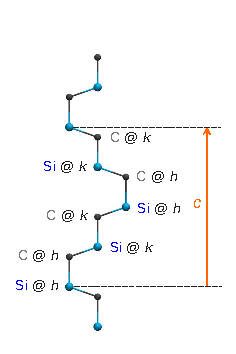
\includegraphics[width=0.38\textwidth]{figures/SiC-non-equiv-sites.pdf}%
        \input{Tikz/MagneticDipole.tex}
  \caption{Schematic of current loop and induced magnetic moment.}%
\end{wrapfigure}%


The \index{magnetic dipole}{magnetic dipole} induces a magnetic field $\vec{B}$, which for points a large distance from the dipole may be calculated as \cite{Griffiths2012-pt}:
\begin{equation}
    \vec{B} = \frac{\mu_0}{4\pi} \frac{1}{r^3} \left[\frac{3(\vec{\mu} \cdot \vec{r}) \cdot \vec{r}}{r^2} - \vec{\mu}\right]
    \label{eq:}
\end{equation}

The symmetry of the field enables us to consider the direction of the dipole as aligned to the $z$-axis. Then, defining $x,y$ as usual by $r \cos\theta$ and $r \sin\theta$ respectively. We may decompose the \index{magnetic field}{magnetic field} in two separate components, parallel ($B_z$) and perpendicular ($B_x, B_y$): 
$$B_\parallel =\frac{\mu_0}{r^3}(3\cos^2 \theta - 1), \quad B_\perp = \frac{3\mu_0}{r^3}\cos\theta\sin\theta.$$
Where we use the Pythagorean principle to determine the overall magnitude $B = |\vec{B}|$ as
$$B = \sqrt{B_\parallel^2 + B_\perp^2}.$$

\subsection{Gyromagnetic Ratio}
\subsubsection{Classical Derivation}
The current in equation \ref{eq:dipole_moment} is proportional to the angular momentum of the charge. That is, the dipole moment is always associated with an angular momentum $\vec{G} = \vec{r} \times \vec{p}$ with $\vec{r}$ the radius and $\vec{p}$ the momentum. 

Dividing the magnetic dipole moment by the angular momentum we find the \textbf{gyromagnetic ratio}. 
\begin{equation}
    \gamma = \frac{\vec{\mu}}{\vec{G}}.
    \label{eq:gyromagnetic_ratio}
\end{equation}

Without loss of generality we may consider the most simple case which is where the magnetic dipole moment is parallel (or anti-parallel) to the angular momentum. Then we may consider the absolute values for the dipole moment and the angular momentum: 
\begin{equation}
    \mu = IS, \quad I = 
    % \underbrace{\frac{q}{2\pi R}}_{\rho \text{ (charge density)}}v,
    \frac{qv}{2\pi R},
    \quad S = \pi R^2 
    % \label{eq:}
\end{equation}
We substitute $I$ and $S$ to find 
\begin{equation}
    \mu = \frac{qvR}{2} 
    % \label{eq:}
\end{equation}
% which we substitute into our equation for the gyromagnetic ratio 
% \begin{equation}
%     \gamma = \frac{\frac{qvR}{2}}{\vec{G}}. 
%     \label{eq:789}
% \end{equation}
and further, we equate the angular momentum vector, using the model of a planar loop to 
\begin{equation}
   G= m_q v R 
    % \label{eq:}
\end{equation}
leaving 
\begin{equation}
    \gamma = \frac{q}{2m_q } . 
    % \label{eq:}
\end{equation}

We finally consider that we may represent the, currently unknown, charge and mass as a sum of electron charges and masses. 
\begin{equation}
    \gamma = \frac{q}{2m_q } = \frac{\cancel{N}e}{2\cancel{N} m_e} \implies \gamma = \frac{e}{2 m_e}
    \label{eq:gyromagnetic_ratio}
\end{equation}

We therefore find that the gyromagnetic ratio of the electron depends only on fundamental constants \cite{bromley2000quantum}.

%pg 329 
% https://www.google.co.uk/books/edition/_/7qCMUfwoQcAC?hl=en&gbpv=1&bsq=walter%20greiner%20theoretical%20physics



\subsubsection{Extending to Quantum Mechanics}
Since the gyromagnetic ratio was calculated considering the motion of dipole in a loop, we may extend this to an electron in an orbit.

\begin{wrapfigure}{r}{0.5\textwidth}%
	% \centering%
	\begin{center}
		% 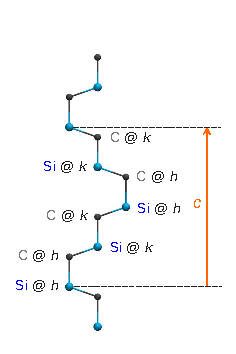
\includegraphics[width=0.38\textwidth]{figures/SiC-non-equiv-sites.pdf}%
		\input{Tikz/OrbitalMagneticMoment.tex}
		\caption{Schematic of electron in orbit generating a magnetic moment.}%
	\end{center}
\end{wrapfigure}%
The fundamental change required to extend the model to quantum mechanics is the treatment of angular momentum which should now be quantised.
Thus, we replace our classical approximation of $\vec{G} = \vec{r} \times \vec{p}$ with the equation for the eigenvalues of the quantum mechanical representation of orbital angular momentum,
\begin{equation}
	\hat{G} = \hbar \hat{L}
	\label{eq:orbital_angular_momentum}
\end{equation}
where $\hat{L}$ is the operator of the orbital angular momentum (quantum number of orbital momentum).
The angular momentum and total energy are conserved in general in a closed system.

We consider the time independent \index{Shr\"odinger equation}{Shr\"odinger equation}
\begin{equation}
	\hat{H} \Psi_n = E_n \Psi_n
	\label{eq:TISE}
\end{equation}

and choose $\Psi_n$ such that it is an eigenfunction of the Hamiltonian, the total angular momentum squared ($L^2 = L_x^2 + L_y^2 + L_z^2$) and exactly one directional component of the angular momentum which is by convention chosen as $L_z$.

According to quantum mechanics the projection of $L$ along the \index{quantisation axis} ($m_L$) may take integer values $-L, -L + 1, \dots, L-1, L$.
Thus, we may describe a given quantum state by the angular momentum $L$ and it's projection $m_L$. Thus, using \index{Dirac notation}{Dirac Notation} we write
\begin{eqnarray}
	&\hat{H}\ket{L, m_L} &= E\ket{L, m_L} \\
	&\hat{L^2}\ket{L, m_L} &= L(L+1)\ket{L, M_L} \\
	&\hat{L_z}\ket{L, m_L} &= m_L\ket{L, m_L}. \label{eq:zthcomponent}
\end{eqnarray}
Thus, the operator which describes the orbital magnetic moment may be written using  \eqref{eq:gyromagnetic_ratio_electrons}, \eqref{eq:orbital_angular_momentum} as
\begin{equation}
	\hat{\vec{\mu}}_L = \gamma \hat{\vec{G}}_L = \gamma \hbar \hat{\vec{L}} = \frac{e\hbar}{2m_e c}\hat{\vec{L}}.
	\label{eq:orbital_magnetic_moment_operator}
\end{equation}

This leads to a quantity known as the \textbf{\index{Bohr magneton}{Bohr Magneton}}, $\mu_B$, given by \cite{Ramamurti1995-wg}
\begin{equation}
	\mu_B = \frac{|e|\hbar}{2m_e c}.
	\label{eq:bohr_magneton}
\end{equation}

Using this we may write \eqref{eq:orbital_magnetic_moment_operator} as
\begin{equation}
	\hat{\vec{\mu}}_L = -\mu_B\hat{\vec{L}}.
	\label{eq:orbital_magnetic_moment_operator_bohr_magneton}
\end{equation}


\subsection{g-factor}
The above expression is valid for the orbital electron but may be extended to a more general system by introducing a \index{g-factor}{g-factor}. The g-factor is equivalent to a dimensionless gyromagnetic ratio \cite{giancoli2008physics}, so \eqref{eq:orbital_magnetic_moment_operator_bohr_magneton} may be written with $g=1$ as
\begin{equation}
	\hat{\vec{\mu}}_L = -g\mu_B\hat{ \vec{L}}.
	\label{eq:orbital_magnetic_moment_operator_bohr_magneton_g_factor}
\end{equation}





% \section{Land\'e g-factor}
\lipsum[1-3]

\section{Spin}
The magnetic moment of elementary particles is called spin. 

% Dirac Equation 

% Pauli Equation 



\section{Zeeman Effect}\label{zeeman}
When no magnetic field is applied to a system, the magnetic dipoles of the orbital electron and spin have no preferred direction. 
The energy levels for all combinations of $L$ and $S$ (all $J$) are equivalent. 

If a magnetic field is applied the magnetic moments interact with that field via the \index{Zeeman!Zeeman interaction}. 
The \index{Zeeman!Zeeman effect} consists of atomic energy level splitting when an external magnetic field is imposed on a sample \cite{Nabokov2002}. 

The classical expression for the energy of a dipole in a magnetic field
\begin{equation}
    E = -\vec{\mu}\cdot\vec{B}
    \label{eq:}
\end{equation}
may be replaced with the Hamiltonian for a quantum mechanical system 
\begin{equation}
    \hat{H}_{\text{Zeeman}} = - \hat{\vec{\mu}}\cdot \vec{B}. 
    \label{eq:}
\end{equation}

The negative sign indicates that when the magnetic moment is parallel to the magnetic field the lowest energy is achieved. 

Thus distinct quantum systems with different $J$ and thus different projections of angular momentum ($m_J$) have different energies due to their interaction with a magnetic field. 

Considering a simple two-level system ($S=1/2$), the energy difference between the spin being aligned or anti-aligned with the field is called the Zeeman energy. 

The Hamiltonian to describe the energy is, using the total angular momentum form of \eqref{eq:orbital_magnetic_moment_operator_bohr_magneton_g_factor}, 
\begin{equation}
    \hat{H}_{\text{Zeeman}} = g \mu_B \hat{\vec{S}}\cdot\vec{B}. 
    \label{eq:}
\end{equation}

Without loss of generality we may direct the magnetic field along the $z$ axis and reduce the scalar product to only the $z$ component. Now, using $S=1/2$ quantised along the $z$ axis, i.e. $m_S = \pm 1/2$ we find the Zeeman energy by solving the Shr\"odinger equation 
\begin{equation}
    \hat{H}_{\text{Zeeman}} \ket{S, m_S} = E_{\text{Zeeman}}\ket{S, m_S} 
    % \label{eq:}
\end{equation}
which, to a factor is equivalent to, by \eqref{eq:zthcomponent}, to
\begin{equation}
    \hat{S}_{z} \ket{S, m_S} = m_S\ket{S, m_S}.
    % \label{eq:}
\end{equation}

Thus we find the two eigenvalues to be
$$E_+ =\frac{1}{2}g\mu_BB, \qquad E_-=-\frac{1}{2}g\mu_BB$$
and thus the Zeeman energy is given by $g\mu_B B$. 

The $S=1/2$ system is thus doubly \index{degenerate} and the \index{degeneracy} is lifted by the application a magnetic field. The Zeeman energy is the difference between the two states and it grows linearly with $B$. 

This may be generalised to a more complex system by considering the total angular momentum $J$ where the energy difference between states is given by 
\begin{equation}
   \Delta E = g_J \mu_B B. 
    \label{eq:zeeman_energy}
\end{equation}






\section{Spin-Orbit Interaction}
The orbital magnetic dipole may interact with the intrinsic spin magnetic dipole via the \index{spin-orbit interaction}{spin-orbit interaction}. This is represented by the spin-orbit Hamiltonian with $\lambda$ representing the constant of the coupling: 
\begin{equation}
    H_{\ce{SO}} = \lambda \hat{\vec{L}}\cdot\hat{\vec{S}}. 
    \label{eq:spin_orbit_hamiltonian}
\end{equation}

This is caused by the interaction between the magnetic field generated by the relativistic motion of the electron around the nucleus and that of the spin magnetic moment. The coupling is proportional to the atomic mass. 


\section{Perturbation Theory}
By considering a ground, non-degenerate state and a \index{perturbation}{perturbation} in the electron Zeeman interaction and the spin-orbit coupling we can develop insight into so called \index{ZFS!zero field splitting}{zero field splitting}. The perturbation is given by 
\begin{equation}
    \hat{H}' = \hat{H}_{\ce{Zeeman}} + \hat{H}_{\ce{SO}}  
    % \label{eq:}
\end{equation}
for which we find 
\begin{equation}
    E_0 = E^{(0)}_0 + \bra{0}{\hat{H}'}\ket{0}  + \sum_{n}\frac{\bra{0} \hat{H}' \ket{n} \bra{n} \hat{H'}\ket{0}}{E_0^{(0)} - E_n^{(0)}}.
    \label{eq:perturbation}
\end{equation}

Now, if we consider arbitrary interactions of forms
\begin{eqnarray}
    &\hat{H}_{\ce{Zeeman}} &= g_L \mu_B \hat{\vec{L}}\cdot\vec{B} + g_S \mu_B \hat{\vec{S}}\cdot\vec{B} \label{eq:zeeman_perturbation}\\ 
    & \hat{H}_{\ce{SO}} &= \lambda\hat{\vec{L}}\cdot \hat{\vec{S}} \label{eq:SO_perturbation}
\end{eqnarray}
we may compute the first and second order corrections. 


\subsubsection{First Order}
Substituting \eqref{eq:zeeman_perturbation} and \eqref{eq:SO_perturbation} into \eqref{eq:perturbation} and integrating only over the orbital values to deduce the Spin Hamiltonian we find
\begin{equation}
   \begin{align}
       \bra{0} \hat{H}' \ket{0} &= \bra{0} g_L \mu_B \hat{\vec{L}}\cdot \vec{B} + g_S \mu_B \hat{\vec{S}}\cdot \vec{B} + \lambda\hat{\vec{L}} \cdot \hat{\vec{S}} \ket{0}\\ 
                                & = \bra{0} g_L\mu_B \hat{\vec{L}} \cdot \vec{B} \ket{0} + \bra{0}g_S \mu_B \hat{\vec{S}}\cdot \vec{B}\ket{0} + \bra{0}\lambda\hat{\vec{L}} \cdot \hat{\vec{S}} \ket{0}\\
                                &= g_L\mu_B \vec{B} \cdot \bra{0}\hat{\vec{L}}\ket{0} + g_S \mu_B  \vec{B} \cdot \hat{\vec{S}}\braket{0|0} + \lambda \hat{\vec{S}} \cdot \braket{0|\hat{\vec{L}}|0}\\ 
                                &= g_L\mu_B \vec{B} \cdot \cancelto{0}{\bra{0}\hat{\vec{L}}\ket{0}} + g_S \mu_B  \vec{B} \cdot \hat{\vec{S}}\cancelto{1}{\braket{0|0}} + \lambda \hat{\vec{S}} \cdot \cancelto{0}{\braket{0|\hat{\vec{L}}|0}}\\ 
                                &= g_s \mu_B \hat{S}\cdot\hat{B}.
   \end{align} 
    \label{eq:first_order}
\end{equation}

Here we used the fact that $\braket{0 | \hat{\vec{L}} | 0} = 0$ since, for example in the alegbraic basis $\hat{L}_z = -i\left(x \frac{\partial}{\partial y} - y \frac{\partial }{\partial x}\right)$ is a Hermitian operator is therefore has eigenvalues which are strictly real numbers, i.e. 
\begin{equation}
    \hat{L}_z \ket{\psi} = m_L \ket{\psi}.
    \label{eq:hermitian}
\end{equation}

By considering \eqref{eq:hermitian} we see that if we apply an imaginary operator to a real valued eigenfunction the corresponding eigenvalue must be imaginary or zero. We know the state is strictly real since it is \index{degeracy!non-degenerate}{non-degenerate}\footnote{A complex wavefunction $\psi$ is at least doubly degenerate; the complex conjugate $\psi^*$ has the same energy.}. In this case, the expectation value of $\hat{L}$ can only be $0$. 

\paragraph{Zeeman Splitting.}
The result of the first order perturbation is thus a more formal confirmation of the result of section \ref{zeeman}, specifically \eqref{eq:zeeman_energy}.  

% Using this we find for some real number $r$ 
% \begin{equation}
%     \hat{L}_z \ket{\psi} \implies \braket{\hat{L}_z | \psi | \hat{L}_z} = r \braket{\psi | \psi}
%     % \label{eq:}
% \end{equation}
% which when applied above gives 
%
\subsubsection{Second Order}
At second order, again substituting \eqref{eq:zeeman_perturbation} and \eqref{eq:SO_perturbation} into \eqref{eq:perturbation} 
and integrating only over the orbital values 
we find 
\begin{equation*}
   \begin{align}
       &\sum_{n}\frac{\bra{0} \hat{H}' \ket{n} \bra{n} \hat{H'}\ket{0}}{E_0^{(0)} - E_n^{(0)}}
   \end{align}
\end{equation*}
\begin{equation}
    \begin{align}
 &=\frac{\braket{0 |g_L \mu_B \hat{\vec{L}}\cdot\vec{B} + g_S \mu_B \hat{\vec{S}}\cdot\vec{B} +\lambda\hat{\vec{L}}\cdot \hat{\vec{S}}  | n } \braket{n |g_L \mu_B \hat{\vec{L}}\cdot\vec{B} + g_S \mu_B \hat{\vec{S}}\cdot\vec{B}+\lambda\hat{\vec{L}}\cdot \hat{\vec{S}}| 0}}{E_0^{(0)} - E_n^{(0)}}\\ 
 &=\frac{\braket{0 |g_L \mu_B \hat{\vec{L}}\cdot\vec{B} + \lambda\hat{\vec{L}}\cdot \hat{\vec{S}}  | n } \braket{n |g_L \mu_B \hat{\vec{L}}\cdot\vec{B} + \lambda\hat{\vec{L}}\cdot \hat{\vec{S}}| 0}}{E_0^{(0)} - E_n^{(0)}}\\ 
 &= (g_L \mu_B \vec{B} + \lambda \hat{\vec{S}})\underbrace{\sum_n \frac{\braket{0 |\hat{\vec{L}} | n}\braket{n |\hat{\vec{L}} | 0}}{E_0^{(0)} - E_n^{(0)}}}_{{\Lambda}}(g_L \mu_B \vec{B} + \lambda \hat{\vec{S}})%
    \end{align}
    % \label{eq:}
\end{equation}

Here $\Lambda$ is a matrix composed of the elements as shown. Expanding out, this allows us to write the second order perturbation as 
\begin{equation}
    \sum_{n}\frac{\bra{0} \hat{H}' \ket{n} \bra{n} \hat{H'}\ket{0}}{E_0^{(0)} - E_n^{(0)}} = g_L^2\mu_B^2 \vec{B} \cdot \Lambda \cdot \vec{B} + 2\lambda g_L\mu_B\hat{\vec{S}}\cdot\Lambda\cdot\vec{B} + \lambda^2 \hat{\vec{S}}\cdot \Lambda \cdot \hat{\vec{S}}.
    \label{eq:second_order}
\end{equation}

Since for EPR we are only interested in the spin-dependent terms, the first term may be neglected as it represents a global shift in the energy spectra. 

\subsubsection{Combined Perturbation}
Combining \eqref{eq:first_order} and \eqref{eq:second_order} we find 
\begin{equation}
    \begin{align}
    \bra{0} \hat{H}' \ket{0}+  \sum_{n}\frac{\bra{0} \hat{H}' \ket{n} \bra{n} \hat{H'}\ket{0}}{E_0^{(0)} - E_n^{(0)}}
    &= g_S \mu_B \hat{\vec{S}} \cdot \vec{B} + 2\lambda g_L\mu_B\hat{\vec{S}}\cdot\Lambda\cdot\vec{B} + \lambda^2 \hat{\vec{S}}\cdot \Lambda \cdot \hat{\vec{S}} \\ 
    &=\mu_B \hat{\vec{S}} \cdot \underbrace{(g_S + 2g_L \lambda \Lambda)}_{g} \cdot \vec{B} + \hat{\vec{S}}\cdot \underbrace{\lambda^2 \Lambda}_{D} \cdot \hat{\vec{S}}.
    \end{align}
    \label{eq:}
\end{equation}
In this expression $g$ and $D$ are matrix quantities depending on $\Lambda$ and represent the (possibly anisotropic) $g$ factor and $D$ the fine structure splitting. 

{\color{red}For this work we will consider only systems in which the differences in angular momentum is due only to the spin and thus $g$ is reduced to a scalar quantity in the spin Hamiltonian.\td{More like - we consider $g$ to be isotropic and symmetric} 
}

The term depending on $D$ has no dependence on magnetic field and thus this \index{fine-structure}{fine-structure} splitting is known as zero field splitting (ZFS) and is observed in systems with $S > 1/2$. 
\begin{equation}
    H_{\ce{FS}} = \hat{\vec{S}}\cdot D \cdot \hat{\vec{S}}. 
    \label{eq:fine_structure}
\end{equation}








    % %Dipole 
%Fermi Contact



    % The same thing?
    % develop then explain why we disregard
% After introducing then cover ZFS (page 80+ PAvel book)
\section{Zero Field Splitting}\label{zfs}
\index{ZFS}{ZFS} is in fact due to the combined effects of fine structure and a dipole-dipole interaction. These effects manifest themselves identically which makes them difficult to separate experimentally. They each depend on a traceless matrix $D$, as will be shown, which can be totally described by two parameters, conventionally labelled $D$ and $E$. 
For simplicity in this work we will consider the combined effect of both the fine-structure and the dipole-dipole interaction as the ZFS interaction. This means when $D$ and $E$ are measured for a specific system, they represent the compound effect of fine-structure splitting and the dipole interaction, but totally describe the zero-field splitting. 

\begin{figure}[H]
    \begin{center}
        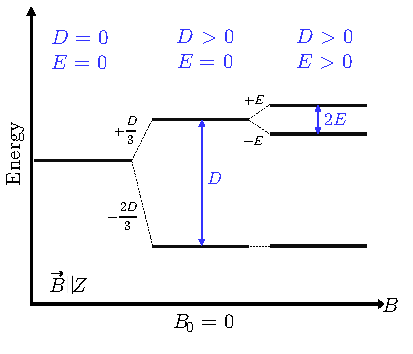
\includegraphics[width=0.6\textwidth]{figures/ZFS.pdf}
    \end{center}
    \caption{Adapted from figure shown in the work by Gr\"{u}ne. }\label{fig:ZFS}
\end{figure}



\subsection{Fine Structure}
The matrix $D$ in \eqref{eq:fine_structure} has form 
\begin{equation}
   D = \begin{pmatrix}
       D_{xx} & D_{xy} & D_{xz} \\ 
       D_{yx} & D_{yy} & D_{yz} \\ 
       D_{zx} & D_{zy} & D_{zz} \\ 
   \end{pmatrix} 
    % \label{eq:}
\end{equation}
which may be simplified by alignment to the wider system axis and diagonalising the matrix as 
\begin{equation}
   D = \begin{pmatrix}
       D_{xx} & 0 & 0 \\ 
       0 & D_{yy} & 0 \\ 
       0 & 0 & D_{zz} \\ 
   \end{pmatrix}.
    \label{eq:fine_splitting_D}
\end{equation}

The \index{trace}{trace} of the matrix $\text{Tr}(D)$ is unchanged by the change of basis. Since for EPR we are only concerned with the changes in energy and not the absolute, we may choose the value of the trace without any loss of generality, so we set it equal to zero. 
\begin{equation}
    \text{Tr}(D) = 0. 
    % \label{eq:}
\end{equation}

This means that the diagonal form of $D$ may be fully determined by just two parameters 
\begin{eqnarray}
    &D &= D_{zz} - (D_{xx}+ D_{yy})/2 \label{fs_D}\\ 
    &E &= (D_{xx} - D_{yy})/2 \label{fs_E}
\end{eqnarray}

Here $D$ represents the axially symmetric parameter and $E$ represents any non-axial contribution of the fine-structure interaction. 

Substituting \eqref{fs_D} and \eqref{fs_E} into \eqref{eq:fine_structure} and expanding allows us to write our fine-structure Hamiltonian as
\begin{equation}
    H_{\ce{FS}} = D \left(\hat{S}_z^2 - \frac{1}{3}S(S+1)\right) + E\left(\hat{S}_x^2 - \hat{S}_y^2\right).
    \label{eq:fine_structure_hamiltonian}
\end{equation}

\subsection{Dipole-Dipole Interaction}
We will now show that the interaction between the magnetic dipoles of two electrons has the same form as \eqref{eq:fine_structure} by considering two electrons ($S=1/2$). 

We begin with the classical expression for the energy between two magnetic dipoles, $\mu_1, \mu_2$
\begin{equation}
    E = \frac{1}{r^3} \left(\mu_1 \cdot \mu_2 -\frac{3(\mu_1 \cdot \vec{r})(\mu_2 \cdot \vec{r})}{r^2}\right).
    % \label{eq:}
\end{equation}

Substituting the quantum mechanical operators for the two electron magnetic dipoles we find 
\begin{equation}
    H_{\ce{DD}} = g_S^2 \mu_B^2 \frac{1}{r^3} \left(\hat{\vec{S}}_1 \cdot \hat{\vec{S}}_2 -\frac{3(\hat{\vec{S}}_1 \cdot \vec{r})(\hat{\vec{S}}_2 \cdot \vec{r})}{r^2}\right).
    % \label{eq:}
\end{equation}

Considering the total spin of the system we may expand this to obtain \cite{carrington1967introduction} 
\begin{equation}
    H_{\ce{DD}} = \frac{1}{2r^5}g_S^2 \mu_B^2 \hat{\vec{S}} \cdot
    \underbrace{
    \begin{pmatrix}
        {r^2 - 3x^2} & -3xy & - 3xz\\ 
        -3xy & r^2 - 3y^2 & -3yz \\ 
        -3xz & -3yz & r^2 - 3z^2 
    \end{pmatrix}
}_{D}
    \cdot \hat{\vec{S}}.
    \label{eq:dd_matrix_form}
\end{equation}

As with \eqref{eq:fine_splitting_D} the matrix $D$ in \eqref{eq:dd_matrix_form} has a constant trace (which we may select to be $0$) leaving the form of the dipole-dipole interaction identical to that of the fine structure interaction 

\begin{equation}
    H_{\ce{DD}} = \hat{\vec{S}} \cdot D \cdot \hat{\vec{S}}.
    % \label{eq:}
\end{equation}

We therefore decompose the traceless matrix $D$ into the axial and non-axial parameters \index{ZFS!$D$}{$D$} and \index{ZFS!$E$}{$E$} as above. 


\subsection{Zero Field Splitting Hamiltonian}
When measuring the values of $D$ and $E$ experimentally, the combined effect will be contained within those measurements so we may therefore describe the zero field splitting interaction as a whole using 
\begin{equation}
    H_{\ce{ZFS}} =D \left(\hat{S}_z^2 - \frac{1}{3}S(S+1)\right) + E\left(\hat{S}_x^2 - \hat{S}_y^2\right).
    \label{eq:ZFS_hamiltonian}
\end{equation}

The effects of $D$ and $E$ on a triplet state are illustrated in Figure~\ref{fig:ZFS}.



% Quardripole? Develop and disregard?
% Nuclear effect - dont even include (or do?)
\section{Nuclear Hamiltonians}

\lipsum[1-4]

% Stark Effect
\section{Stark Effect}
\tdr{Deduce Stark Effect Hamiltonian and write up}
\lipsum[5-8]

%https://journals.aps.org/prl/abstract/10.1103/PhysRevLett.112.087601
\section{Total Hamiltonian}
We now have all the components of our total Hamiltonian for both $S=1$ and $S=3/2$ systems given by
\begin{equation}
   H =  H_{\ce{Zeeman}} + H_{\ce{ZFS}} + H_{\ce{Stark}}
    \label{eq:total_hamiltonian}
\end{equation}
using
\begin{equation}
    H_{\ce{Zeeman}} &= g \mu_B \hat{\vec{S}}\cdot \vec{B}, \tag{\ref{eq:Zeeman_Hamiltonian}}\\ 
\end{equation} 
\begin{equation}
    H_{\ce{ZFS}} &=  D\left(\hat{S}_z^2 - \frac{1}{3}S(S+1)\right)  + E(\hat{S}_x^2 - \hat{S}_y^2),\tag{\ref{eq:ZFS_hamiltonian}}\\ 
\end{equation}

and
\begin{equation}
    H_{\ce{Stark}} &=
                        d_\parallel E_z\left(\hat{S}_z^2 - \frac{1}{3} S(S+1)\right)
                        - d_\perp  E_y(\hat{S}_x^2 - \hat{S}_y^2   ) + d_\perp E_x(\hat{S}_x\hat{S}_y + \hat{S}_y\hat{S}_x).  \tag{\ref{eq:stark_hamiltonian}}
\end{equation}



\section{Spin Hamiltonian}
We can apply \eqref{eq:total_hamiltonian} to our specific $S=1$ or $S=3/2$ system by substitution of the spin operators. They are a matrix representation of the $su(2)$ algebra, equivalent to Pauli matrices in the relevant dimension.
\subsection{$S=1$ Spin Operators}
The three dimensional \index{spin operators!$S=1$}{$S=1$} spin operators $S_j$ in matrix representation are
\begin{equation}
	S_x = \frac{1}{\sqrt{2}} \begin{pmatrix}
		0 & 1 & 0 \\
		1 & 0 & 1 \\
		0 & 1 & 0
	\end{pmatrix},
	S_y = \frac{i}{\sqrt{2}} \begin{pmatrix}
		0 & -1 & 0  \\
		1 & 0  & -1 \\
		0 & 1  & 0
	\end{pmatrix},
	S_z = \frac{1}{\sqrt{2}} \begin{pmatrix}
		1 & 0 & 0  \\
		0 & 0 & 0  \\
		0 & 0 & -1
	\end{pmatrix}.
	\label{eq:s1_spin_operators}
\end{equation}

\subsection{$S=3/2$ Spin Operators}
The four dimensional \index{spin operators!$S=3/2$}{$S=3/2$} spin operators $S_j$ in matrix representation are
\begin{equation}
    \begin{align}
        S_x &= \frac{1}{2} \begin{pmatrix}
            0 & \sqrt{3} & 0 & 0 \\
            \sqrt{3} & 0 & 2 & 0  \\
            0 & 2 & 0 & \sqrt{3} \\ 
            0 & 0 & \sqrt{3} & 0
        \end{pmatrix},&
            S_y &= \frac{1}{{2i}} \begin{pmatrix}
                0 & \sqrt{3} & 0 & 0   \\
                -\sqrt{3} & 0  & 2 & 0 \\
                0 & -2 & 0 & \sqrt{3}\\ 
                0 & 0 & -\sqrt{3} & 0
		\end{pmatrix}, \\
                &
        &S_z = \frac{1}{2} \begin{pmatrix}
            3 & 0 & 0 & 0   \\
            0 & 1 & 0 & 0  \\
            0 & 0 & -1 & 0  \\
            0 & 0 & 0 & -3
		\end{pmatrix}.
        &
    \end{align}
	\label{eq:s1.5_spin_operators}
\end{equation}


\section{Strain and Pressure}
The effect of a strain is treated as an effective electric
field 

% [32] A. E. Hughes and W. A. Runciman, Proceedings of the
% Physical Society 90, 827 (1967).
% [33] G. Davies and M. F. Hamer, Proceedings of the Royal
% Society A: Mathematical, Physical and Engineering Sci-
% ences 348, 285 (1976)


%%%%%%%%%%%%%%%%%%%%%%%%%%%%%%%%%%%%%%%%%%%%%%%%%%%%%%%%%%% TODO LINE %%%%%%%%%%%%%%%%%%%%%%%%%%%%%%%%%%%%%%%%%%%%%

\section{Quantum Sensing}
Quantum sensing involves using a qubit system acting as a quantum sensor that interacts with an external variable of
interest, such as a magnetic field, electric field, strain or acoustic wave, or temperature \cite{Castelletto_2024}. 

Quantum sensors have a higher sensitivity within a nanoscale or microscale sampling volume compared to a fully classical counterpart which would require higher field densities or higher volume interrogation to be effective. 

% Quantum sensing, for example, uses the spin state to acquire a phase shift from interactions with the environment10, and an optical interface (that is, spin-to-photon conversion) allows optical readout of a spin qubit, potentially enhanced by spin-to-charge conversion
\cite{Wolfowicz2021}

% Quantum sensors detect weak physical signals in nanoscale by quantum coherence, quantum properties or quantum entanglement. 
\cite{Kin2021}


% Unlike heritage designs, the magnetometer does not require inductive sensing elements, high frequency radio, and/or optical circuitry and can be made significantly more compact and lightweight,
%....
%Additionally, the robustness of the SiC semiconductor allows for operation in extreme conditions
\cite{Cochrane2016}


% We achieve two-spin interference with a phase sensitivity of 1.79 ± 0.06 dB beyond the SQL and three-spin interference with a phase sensitivity of 2.77 ± 0.10 dB. Besides, a magnetic sensitivity of 0.87 ± 0.09 dB beyond the SQL is achieved by two-spin interference for detecting a real magnetic field. Particularly, the deterministic and joint initialization of NV negative state, NV electron spin, and two nuclear spins is realized at room temperature. The techniques used here are of fundamental importance for quantum sensing and computing, and naturally applicable to other solid-state spin systems.
\cite{Xie2021}

% \paragraph{Qubits}
% A quantum bit or qubit is a simple quantum mechanical system with two eigenstates. 

\subsection{DiVincenzo Criteria}
To construct a working quantum sensor with any candidate system, DiVincenzo and Degen outlined a set of three necessary conditions that must be followed \cite{Crawford2021, RevModPhys.89.035002, DiVincenzo1995}

\begin{enumerate}
    \item The quantum system must have discrete resolvable energy levels (or an ensemble of two-level systems with a lower energy state $\ket{0}$ and an upper energy state $\ket{1}$) that are separated by a finite transition energy. 
    \item It must be possible to initialise the quantum sensor into a well-known state and to read out its state. 
    \item The quantum sensor can be coherently manipulated, typically by time-dependent fields.
\end{enumerate} 

Spin defects are mostly paramagnetic and radiative point defects (or colour centres). Colour centres possessing a 
non-zero electron spin are excellent candidates for optical spin
quantum bits (qubits) \cite{Castelletto_2024}.

Colour centres can produce detectable luminescence even at room temperature. Optical radiation is generally used as a readout but the excitation can also be used for spin manipulation and control.


\cite{RevModPhys.89.035002}
% To construct a working quantum sensor with any candidate material, DiVincenzo[39] and Degen[6] outlined a set of three necessary conditions that must be followed: i) The quantum system must have discrete resolvable energy levels (or an ensemble of two-level systems with a lower energy state |0⟩ and an upper energy state |1⟩) that are separated by a finite transition energy; ii) it must be possible to initialize the quantum sensor into a well-known state and to read out its state; iii) the quantum sensor can be coherently manipulated, typically by time-dependent fields.
\cite{Crawford2021}

\subsection{Crystal Defects}
% Because of about 250 SiC polytypes are known, there should exist more than thousand different spin defects in SiC with distinct characteristics14,15. One can select defects with the most suitable properties for a concrete task, which is not possible for one universal sensor.

\cite{Kraus2014}

% Spin defect centers with long quantum coherence times (T2) are key solid-state platforms for a variety of quantum applications. 
\cite{Kanai2022}

\subsubsection{Quantisation}
\subsubsection{Polarisation}
 % Based on magnetic-dipole forbidden spin transitions, this scheme enables spatially confined spin control, the imaging of GHz-frequency electric fields, and the characterization of defect spin multiplicity
\cite{PhysRevLett.112.087601}

\subsubsection{Coherent Manipulation}
\cite{Widmann2014}

% We find that simultaneous optical reionization and qubit manipulation can be carried out at room temperature with photoexcitation at the typical excitation wavelength used for readout of the divacancy qubits in 4H SiC
\cite{PhysRevB.105.165108}

% These spin defects can be optically addressed and coherently controlled even at room temperature, and their fluorescence spectrum and optically detected magnetic resonance spectra are different from those of any previously discovered defects. Moreover, the generation of these defects can be well controlled by optimizing the annealing temperature after implantation. These defects demonstrate high thermal stability with coherently controlled electron spins, facilitating their application in quantum sensing and masers under harsh conditions.
\cite{Yan2020}


% These defects are optically active near telecommunication wavelengths11, and are found in a host material for which there already exist industrial-scale crystal growth12 and advanced microfabrication techniques13. In addition, they possess desirable spin coherence properties that are comparable to those of the diamond nitrogen–vacancy centre. This makes them promising candidates for various photonic, spintronic and quantum information applications that merge quantum degrees of freedom with classical electronic and optical technologies
\cite{Koehl2011}

% Coherent manipulation of NV centers in SiC has been achieved with Rabi and Ramsey oscillations. 
\cite{Mu2020}


% Hence, coherent control of NV center spins is achieved at room temperature, and the coherence time 𝑇2 can be reached to around 17.1  𝜇⁢s. Furthermore, an investigation of fluorescence properties of single NV centers shows that they are room-temperature photostable single-photon sources at telecom range.
\cite{PhysRevLett.124.223601}

\subsubsection{Efficient Readout}
% Overcoming poor readout is an increasingly urgent challenge for devices based on solid-state spin defects, particularly given their rapid adoption in quantum sensing, quantum information, and tests of fundamental physics. 
% Our results pave a clear path to achieve unity readout fidelity of solid-state spin sensors through increased ensemble size, reduced spin-resonance linewidth, or improved cavity quality factor.

\cite{Eisenach2021}

% we demonstrate the first ever implementation of SCC for VV0 in SiC by performing spin-selective ionization followed by all-optical single-shot readout of the charge state. Using this technique, we can determine an initially prepared spin state with over 80% fidelity. 
\cite{Anderson2022-sf}


% Here, we demonstrate a photo-electrical detection technique for electron spins of silicon vacancy ensembles in the 4H polytype of silicon carbide (SiC). Further, we show coherent spin state control, proving that this electrical readout technique enables detection of coherent spin motion. Our readout works at ambient conditions, while other electrical readout approaches are often limited to low temperatures or high magnetic fields.
\cite{Niethammer2019}


% High-fidelity single-shot spin readout in silicon opens the way to the development of a new generation of quantum computing and spintronic devices, built using the most important material in the semiconductor industry.
\cite{Morello2010}

% Even if the signal-to-noise ratio is reasonably low, a well-trained convolutional neural network (CNN) can predict the resonance peaks of ODMR spectra or the period of Rabi oscillations. Because of the fast output of predictions by the CNN, this method can be used to sense the magnetic field in the environment and microwave intensities in real time.
\cite{PhysRevApplied.17.034046}


\subsection{Coherence}
\cite{Christle2014},\cite{Soltamov2019}, \cite{Gilardoni2020} \cite{BulanceaLindvall2021}, \cite{Astner2022}

% Long coherence times are key to the performance of quantum bits (qubits). 
\cite{Seo2016-ed}

\subsubsection{Spin Relaxation}
\subsubsection{Dephasing}
\subsubsection{Hahn Echo}
% The coherence time of NV defects in the presence of noise originating from parasitic spins located at the diamond interface can be improved by orders of magnitude by using high-order spin echoes.
\cite{Wu2016}
\subsubsection{Example: NV Diamond}


\subsection{Sensitivity}
\cite{RevModPhys.92.015004}

% Our approach is suitable for ensemble as well as single spin-3/2 color centers, allowing for angle-resolved magnetometry on the nanoscale at ambient conditions.
\cite{PhysRevApplied.4.014009}


 % We report the realization of nanotesla shot-noise-limited ensemble magnetometry based on optically detected magnetic resonance with the silicon vacancy in 4⁢𝐻 silicon carbide. By coarsely optimizing the anneal parameters and minimizing power broadening, we achieve a sensitivity of 50nT/√Hz and a theoretical shot-noise-limited sensitivity of 3.5nT/√Hz.
\cite{PhysRevApplied.15.064022}

% By inserting an NV-doped diamond membrane between two ferrite cones in a bowtie configuration, we realize a ∼250-fold increase of the magnetic field amplitude within the diamond. We demonstrate a sensitivity of ∼0.9⁢pTs1/2 to magnetic fields in the frequency range between 10 and 1000Hz. 
\cite{PhysRevResearch.2.023394}


% For all these color centers we saw an enhancement of the photostable fluorescence emission of at least a factor of 6 using micro-photoluminescence systems. Using custom confocal microscopy setups, we characterized the emission of VSi measuring an enhancement by up to a factor of 20, and of NCVSi with an enhancement up to a factor of 7. The experimental results are supported by finite element method simulations. Our study provides the pathway for device design and fabrication with an integrated ultra-bright ensemble of VSi and NCVSi for in vivo imaging and sensing in the infrared.
\cite{Castelletto2019}

 % low photon count rate significantly limits their applications. We strongly enhanced the brightness by 7 times and spin-control strength by 14 times of single divacancy defects in 4H-SiC membranes using a surface plasmon generated by gold film coplanar waveguides.
\cite{Zhou2023}

\begin{group}
\color{lightgray}
Most of the SiC colour centres have a residual spin and
therefore all could be in principle used in quantum sens-
ing. However, they can be distinguished and grouped by their
ground state spin value and the zero field (magnetic) split-
ting (ZFS), which defines their properties and the different
methods for their initialisation, control, and read-out. Colour
centres with the high-spin ground state (S = 1, 3/2) can be
used as two or three levels quantum systems (figure 1(c)). They
can be controlled optically and using a microwave (MW) or
radio frequency (RF) excitation due to the higher sensitivity to
the presence of the magnetic field.


The spin Hamiltonian of an S = 3/2 elec-
tron spin defect within a nuclear spin bath can be written as:

\begin{equation}
    \hat{H} = \underbrace{g \mu_B \hat{\mathbf{S}} \cdot \mathbf{B}_0}_{H_{\text{Zeeman}}} + D \left( \hat{\mathbf{S}}_z^2 - \frac{S(S+1)}{3}\right) + E (\hat{\mathbf{S}}^2_x - \hat{\mathbf{S}}^2_y) + \sum_j \hat{\mathbf{S}}_i \cdot \mathbf{A}_{ij} \cdot \hat{\mathbf{I}}_j
    \label{eq:}
\end{equation}
where g is the isotropic centre specific Lande factor (g =
2.0028), µB is the Bohr magneton, B0 is the external magnetic
field, D and E account for the zero magnetic fields splitting
for the axial (along the spin polarisation axis) or the off-axis
component of the spin defect operator Ŝ = (Sˆx , Sˆy , Ŝz ) respect-
ively. Aij is the hyperfine tensor that describes the central spin
coupling to many nuclear spins indexed by j with spin operat-
ors Iˆj .
\end{group}



\section{Spin Polarisation}\label{spin_polarisation}
\cite{2008}\cite{Weil2006}\cite{Goldfarb2018-he}\cite{Richert2017}
Spin polarisation in the context of EPR is the unequal population of possible spin states. 
For example the differing population of triplet sublevels under the influence of photoexcitation. 
Microwave radiation is only absorbed or emitted in a spin polarised system; so spin polarisation is essential for EPR. 

When the spin is polarised, the unequal population is brought back to equilibrium either by the thermodynamic effect of spin-lattice interactions, or by an induced magnetic resonance transition as is exploited by EPR.

\index{Boltzman statistics}{Boltzman statistics}
% BOLTZMAN STATISTICS

\subsection{Optical Polarisation}
% We find that simultaneous optical reionization and qubit manipulation can be carried out at room temperature with photoexcitation at the typical excitation wavelength used for readout of the divacancy qubits in 4H SiC
\cite{PhysRevB.105.165108}


\section{\index{ODMR}{ODMR}}\label{ODMR}
Optically detected magnetic resonance, specifically continuous wave optically detected magnetic resonance will be the read-out mechanism discussed in this work. This is not necessarily the most sensitive mechanism for any given system, but remains popular due to the very simple implementation. 

The process is to measure the photoluminescence of the spin polarised sample whilst sweeping the driving field to find where the Rabi oscillations occur. When the change of photoluminescence is at a peak, the Rabi frequency is exactly the energy difference between the two spin sub-levels. The energy of and energy difference between the spin sub-levels is dependent on the magnetic and electric field, temperature, pressure and strain. 

\begin{figure}[h]
    \begin{center}
        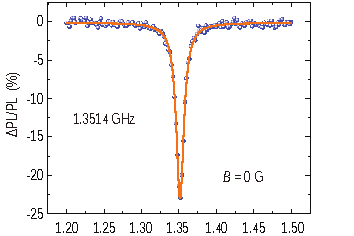
\includegraphics[width=0.5\textwidth]{figures/ODMR.pdf}
    \end{center}
    \caption{
        CW-ODMR spectra for a PL6 defect with $\vec{B} = 0$. Blue dots show data from experiment, the orange line is a Lorentzian fit. Adapted from Li et al.}\label{fig:}
%  CW-ODMR
% spectra in the zero magnetic field. The blue dots are the experimental raw data, and the orange line is the corresponding Lorentzian fitting centred
% at 1.3514 GHz.
    % \cite{Li2021}
    % \todo[inline, color=ediblue]{Write caption}
\end{figure}


Determination of how these physical characteristics influence the change in ODMR spectra is the topic of this work. 


% The results suggest that magnetic field sensing sensitivity can be greatly improved for the optimized laser and microwave power range.
% \cite{PhysRevB.101.064102}


% We measure increased photoluminescence from divacancy ensembles by up to three orders of magnitude using near-ultraviolet excitation, depending on the substrate, and without degrading the electron spin coherence time.
% \cite{Wolfowicz2017}



\section{\index{SiC!Silicon Carbide}{Silicon Carbide}}\label{SiC}

\index{SiC}{SiC} is a semiconductor which can be used for high-power and high temperature electronics \cite{Eddy2009,CASADY19961409}. Many studies have demonstrated SiC's potential as a host material for qubits, which enables the application of SiC quantum sensors even in ambient conditions \cite{PhysRevApplied.6.034001}. Moreover, 
the robustness of SiC allows for operation in extreme conditions
\cite{Cochrane2016}
.

\subsection{Colour Defects in SiC}
Point defects in wide-bandgap semiconductors can have both ground and excited states within the energy gap and, hence, are luminescent centres i.e. colour centres and the luminescence is often stable even at room temperature. 
Many color centers also possess a non-zero electron spin and can be excellent candidates for optical spin qubits \cite{Son2021}.

Multiple colour centres have been observed in SiC, those which may be employed as spin qubits are the divacancy and the Silicon vacancy. 
There are seven types of divacancies in 4H-SiC, the polytype of SiC for which this work will be based. 
The defects can be categorised by their orientation within the lattice. 
These are the c-axis, for which we have the Silicon vacancy V2 and divacancies PL1, PL2, and PL6. 
On the basal axis, we have the divacancies PL3, PL4, PL5, and PL7 \cite{Qin-Yue}. Due to having the highest ODMR contrast 
and coherence at room temperature this work will focus primarily on the c-axis PL6 divacancy and the V2 Silicon vacancy. 
Application of both of these families of defects in quantum sensing can be competitive with the Nitrogen vacancy in diamond \cite{10.1093/nsr/nwab122}.

Figure \ref{fig:SiC_defects} shows the position of the defects in the lattice. 

\begin{figure}[H]
    \begin{center}
        % 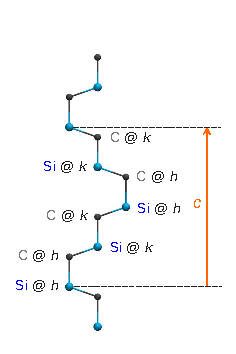
\includegraphics[width=0.32\textwidth]{figures/SiC-non-equiv-sites.pdf}
        % \hspace{1em}
        % 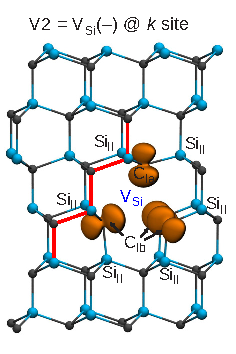
\includegraphics[width=0.32\textwidth]{figures/SiC-V2.pdf}
        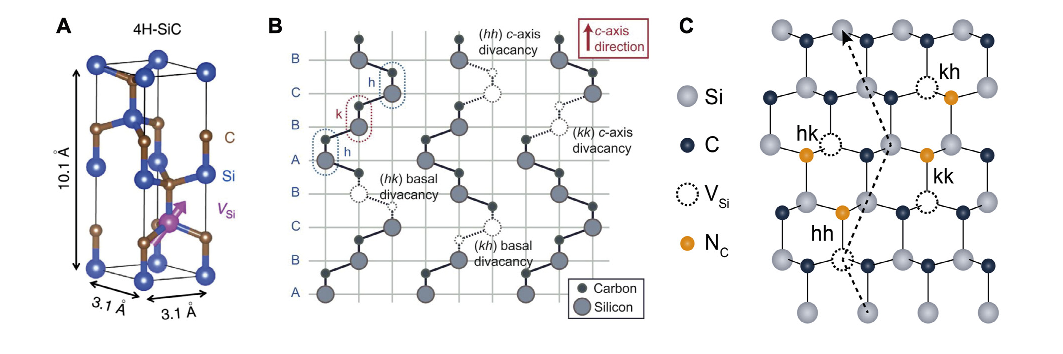
\includegraphics[width=\textwidth]{figures/SiC-lattice.pdf}
    \end{center}
    \caption{(a) Schematic of the 4H-SiC lattice. (b) Possible non-equivalent divacancies sites within the lattice. (c) Schematic of Silicon vacancies within the lattice. Reproduced from Luo et al.}\label{fig:SiC_defects}
    % \cite{Luo2023}
    % \todo[inline, color=ediblue]{Write caption}
\end{figure}



\subsection{Production of SiC}
Whilst the research for the Nitrogen vacancy in diamond is more mature, many equivalent techniques are being developed for 
SiC. 

Diamond is expensive and not compatible with conventional electronic circuits. By comparison, SiC is a technology-friendly material with an existing large-scale production capacity complemented by mature doping techniques \cite{Jiang2023}. Wafer-scale SiC is able to be produced and efficiently manufactured into electronic devices down to the atomic scale \cite{arxiv.1503.07566}.

Divacancies and Silicon vacancies may reliably introduced into SiC. As an example, the Silicon vacancy can be incorporated into the lattice and the density of the vacancies may be controlled down to the single defect level without degradation of the electrical characteristics of the material
\cite{Ohshima2018,PhysRevApplied.4.014009,Wang2019}
.

Further, approaches to manufacture solid-immersion lenses, which may aid the sensitivity or reduce the integration volume of a sensor have been demonstrated
\cite{Sardi2020}
.

Overall, research into the applicability of SiC as a quantum sensor is exciting and shows a lot of potential for application in the near term. 

% we discuss energetic particle irradiation, especially proton beam writing (PBW), in which proton microbeams with MeV range are used, as a method to create VSi in SiC since PBW can create VSi in certain locations with micrometer accuracy and this is very useful to introduce VSi in electronic devices without the degradation of their electrical characteristics.

% Interestingly, VSi can be incorpo-
% rated into SiC nanocrystals [28], and their density can be
% controlled over 8 orders of magnitude down to the single-
% defect level [32].

 % we present the generation and characterization of shallow silicon vacancies in silicon carbide by using different implanted ions and annealing conditions. 

% Here, we demonstrate a scalable approach of manufacturing solid-immersion lenses (SILs) on 4H–SiC.

 
\section{\index{multimodal}{Multimodal Sensing}}
% Using these properties, an integrated magnetic field and temperature sensor can be implemented on the same center.
\cite{Anisimov2016}

 % The effect can be detected as an abrupt reduction of the photoluminescence intensity under optical pumping without application of microwave fields. 
\cite{PhysRevB.100.094104}


% The coherent control of divacancy demonstrates that coherence time decreases as pressure increases. Based on these, the pressure-induced magnetic phase transition of Nd2Fe14B sample at high pressures was detected. These experiments pave the way to use divacancy in quantum technologies such as pressure sensing and magnetic detection at high pressures
\cite{Liu2022}


 % In this paper, we present a self-protected infrared high-sensitivity thermometry based on spin defects in silicon carbide. Based on the conclusion that the Ramsey oscillations of the spin sensor are robust against magnetic noise due to a self-protected mechanism from the intrinsic transverse strain of the defect, we experimentally demonstrate the Ramsey-based thermometry. The self-protected infrared silicon-carbide thermometry may provide a promising platform for high sensitivity and high-spatial-resolution temperature sensing in a practical noisy environment, especially in biological systems and microelectronics systems.
\cite{PhysRevApplied.8.044015}


% Here we show that the defect charge state can also be used to sense the environment, in particular high-frequency (megahertz to gigahertz) electric fields
\cite{Wolfowicz2018}

% we identify the mechanism that polarizes the spin under optical drive, obtain the ordering of its dark doublet states, point out a path for electric field or strain sensing, and find the theoretical value of its ground-state zero-field splitting to be 68 MHz, in good agreement with experiment. Moreover, we present two distinct protocols of a spin-photon interface based on this defect. Our results pave the way toward quantum information and quantum metrology applications with silicon carbide.
\cite{PhysRevB.93.081207}


% We discuss the experimental achievements in magnetometry and thermometry based on the spin state mixing at level anticrossings in an external magnetic field and the underlying microscopic mechanisms. We also discuss spin fluctuations in an ensemble of vacancies caused by interaction with environment.
\cite{Tarasenko2017}

% Moreover, as an example of an application, we demonstrate thermal sensing using the Ramsey method at about 450 K. Our experimental results would be useful for the investigation of high-temperature properties of defect spins and silicon carbide–based broad-temperature-range quantum sensing.
\cite{PhysRevApplied.10.044042}

% The experiments pave the way for the application of silicon carbide-based high-sensitivity thermometers in the semiconductor industry, biology, and materials sciences.
\cite{D3NR00430A}


% The experiment implies the feasibility of using implanted NV centers in high-quality diamonds to detect temperatures in biology, chemistry, materials science, and microelectronic systems with high sensitivity and nanoscale resolution.
\cite{PhysRevB.91.155404}

% . We then use it to detect the strength of an external magnetic field. Finally, we use the Ramsey methods to realize a temperature sensing with a sensitivity of 163.2 mK/Hz1/2. The experiments demonstrate that the compact fiber-coupled divacancy quantum sensor can be used for multiple practical quantum sensing.
\cite{Quan:23}

% These results establish SiC color centers as compelling systems for sensing nanoscale electric and strain fields.
\cite{PhysRevLett.112.087601}




%%%%%%%%%%%%%%%%%%%%%%%%%%%%%%%%%%%%%%%%%%%%%%%%%%%%%%%%%%%%%%%%%%%%%%%%%%%%%%%%%%%%%%%%%%%%%%%%%%%%%%%%%%%%%%%%%%%%




% Consider Including
% \section{To Sort (abstracted)}
% \input{Sections/HahnEcho.tex}
% \input{Sections/SpinBaths.tex}
% \input{Sections/SpinCoupling.tex}
% \section{Defect Orientation}

Colour centres or defects in general are part of the crystal lattice and thus have an associated orientation and direction within the lattice. This allows the definition of a \textbf{defect axis}. For example, in diamond the NV axis is defined as the vector from the vacancy towards the Nitrogen atom when the vacancy is taken as the origin of your co-ordinate system. 

In a tetragonal crystal, due to symmetry there are four possible orientations of a defect within the lattice: $111$, $1\overline{11}$, $\overline{1}1\overline{1}$ and $\overline{11}1$ directions. 

\section{Miller Indices}
The notation for defect orientation above is known as a Miller Index, and we consider the $111$ direction to be aligned with the defect axis. 

This means that if we know the orientation of our crystal then we can establish the orientations of the defect axis inside. For example, using a crystal for which all surfaces belong to the $\{001\}$ lattice planes, each surface normal is aligned with a Cartesian axis. Thus, by fixing the crystal in place, there remain just \textbf{four} possible angles which a defect axis can have with respect to the crystal surface.

Calculating the scalar product of any of the surface planar directions in the family of $\{001\}$ and the four possible orientations of the defect within the lattice we find $\cos\theta = \pm0.6$. Then, considering the physical solutions (from $0, 2\pi$) gives four possible angles that the (directed) defect axis may make with the surface of the crystal: $53.13^\circ$, $306.87^\circ$, $126.9^\circ$ and $233.13^\circ$ ($0.927$, $5.355$, $2.214$ and $4.069$ radians respectively). 






    


% \input{Sections/SpinDetection.tex}
% \input{Sections/SpinRelaxation.tex}
% \input{Sections/DensityMatrices.tex}
% \input{Sections/RabiOscillations.tex}
% \input{Sections/SpinInitialisation.tex}
% \section{Lattice Symmetry}
Tetragonal lattice has the $$

% \input{Sections/StokesShift.tex}
% \section{Linear Combination of Atomic Orbitals}



% \chapter{To Sort}
\section{Spin}
The magnetic moment of elementary particles is called spin. 

% Dirac Equation 

% Pauli Equation 



\section{Zeeman Effect}\label{zeeman}
When no magnetic field is applied to a system, the magnetic dipoles of the orbital electron and spin have no preferred direction. 
The energy levels for all combinations of $L$ and $S$ (all $J$) are equivalent. 

If a magnetic field is applied the magnetic moments interact with that field via the \index{Zeeman!Zeeman interaction}. 
The \index{Zeeman!Zeeman effect} consists of atomic energy level splitting when an external magnetic field is imposed on a sample \cite{Nabokov2002}. 

The classical expression for the energy of a dipole in a magnetic field
\begin{equation}
    E = -\vec{\mu}\cdot\vec{B}
    \label{eq:}
\end{equation}
may be replaced with the Hamiltonian for a quantum mechanical system 
\begin{equation}
    \hat{H}_{\text{Zeeman}} = - \hat{\vec{\mu}}\cdot \vec{B}. 
    \label{eq:}
\end{equation}

The negative sign indicates that when the magnetic moment is parallel to the magnetic field the lowest energy is achieved. 

Thus distinct quantum systems with different $J$ and thus different projections of angular momentum ($m_J$) have different energies due to their interaction with a magnetic field. 

Considering a simple two-level system ($S=1/2$), the energy difference between the spin being aligned or anti-aligned with the field is called the Zeeman energy. 

The Hamiltonian to describe the energy is, using the total angular momentum form of \eqref{eq:orbital_magnetic_moment_operator_bohr_magneton_g_factor}, 
\begin{equation}
    \hat{H}_{\text{Zeeman}} = g \mu_B \hat{\vec{S}}\cdot\vec{B}. 
    \label{eq:}
\end{equation}

Without loss of generality we may direct the magnetic field along the $z$ axis and reduce the scalar product to only the $z$ component. Now, using $S=1/2$ quantised along the $z$ axis, i.e. $m_S = \pm 1/2$ we find the Zeeman energy by solving the Shr\"odinger equation 
\begin{equation}
    \hat{H}_{\text{Zeeman}} \ket{S, m_S} = E_{\text{Zeeman}}\ket{S, m_S} 
    % \label{eq:}
\end{equation}
which, to a factor is equivalent to, by \eqref{eq:zthcomponent}, to
\begin{equation}
    \hat{S}_{z} \ket{S, m_S} = m_S\ket{S, m_S}.
    % \label{eq:}
\end{equation}

Thus we find the two eigenvalues to be
$$E_+ =\frac{1}{2}g\mu_BB, \qquad E_-=-\frac{1}{2}g\mu_BB$$
and thus the Zeeman energy is given by $g\mu_B B$. 

The $S=1/2$ system is thus doubly \index{degenerate} and the \index{degeneracy} is lifted by the application a magnetic field. The Zeeman energy is the difference between the two states and it grows linearly with $B$. 

This may be generalised to a more complex system by considering the total angular momentum $J$ where the energy difference between states is given by 
\begin{equation}
   \Delta E = g_J \mu_B B. 
    \label{eq:zeeman_energy}
\end{equation}






\input{Sections/HahnEcho.tex}
%Dipole 
%Fermi Contact



\input{Sections/SpinBaths.tex}
\section{Spin-Orbit Interaction}
The orbital magnetic dipole may interact with the intrinsic spin magnetic dipole via the \index{spin-orbit interaction}{spin-orbit interaction}. This is represented by the spin-orbit Hamiltonian with $\lambda$ representing the constant of the coupling: 
\begin{equation}
    H_{\ce{SO}} = \lambda \hat{\vec{L}}\cdot\hat{\vec{S}}. 
    \label{eq:spin_orbit_hamiltonian}
\end{equation}

This is caused by the interaction between the magnetic field generated by the relativistic motion of the electron around the nucleus and that of the spin magnetic moment. The coupling is proportional to the atomic mass. 


\subsubsection{Extending to Quantum Mechanics}
Since the gyromagnetic ratio was calculated considering the motion of dipole in a loop, we may extend this to an electron in an orbit.

\begin{wrapfigure}{r}{0.5\textwidth}%
	% \centering%
	\begin{center}
		% 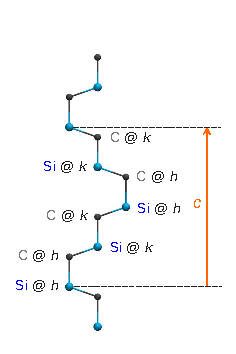
\includegraphics[width=0.38\textwidth]{figures/SiC-non-equiv-sites.pdf}%
		% MAGNETIC MOMENT ATOM
\begin{tikzpicture}[thick, scale=1.5]
  \def\rn{0.3}
  \def\re{0.15}
  \def\Rx{1.5}
  \def\Ry{0.5}
  %\draw[dashed] (-100:1.5*\rn) -- (80:1.5*\rn);
  \draw[dashed] (-\Rx,0) arc (180:0:{\Rx} and {\Ry});
  \draw[mu vector] (0,-1.8*\rn) -- (0,2.9*\rn) node[right] {$\vb*{\mu}$};
  \draw[charge+] (0,0) circle (\rn) node[scale=1.4] {+};
  \draw[dashed] (\Rx,0) arc (0:-180:{\Rx} and {\Ry});
  \draw[charge-]
    (-40:{\Rx} and {\Ry}) circle (\re) node[scale=0.8] {$-$}
    node[below right=0.2] {e};
  \draw[->]
    (-55:{1.15*\Rx} and {1.2*\Ry}) arc (-55:-72:{1.15*\Rx} and {1.2*\Ry});
  \draw[current]
    (-140:{1.15*\Rx} and {1.2*\Ry}) arc (-140:-100:{1.15*\Rx} and {1.2*\Ry})
    node[midway,below] {$I$};
\end{tikzpicture}

		\caption{Schematic of electron in orbit generating a magnetic moment.}%
	\end{center}
\end{wrapfigure}%
The fundamental change required to extend the model to quantum mechanics is the treatment of angular momentum which should now be quantised.
Thus, we replace our classical approximation of $\vec{G} = \vec{r} \times \vec{p}$ with the equation for the eigenvalues of the quantum mechanical representation of orbital angular momentum,
\begin{equation}
	\hat{G} = \hbar \hat{L}
	\label{eq:orbital_angular_momentum}
\end{equation}
where $\hat{L}$ is the operator of the orbital angular momentum (quantum number of orbital momentum).
The angular momentum and total energy are conserved in general in a closed system.

We consider the time independent \index{Shr\"odinger equation}{Shr\"odinger equation}
\begin{equation}
	\hat{H} \Psi_n = E_n \Psi_n
	\label{eq:TISE}
\end{equation}

and choose $\Psi_n$ such that it is an eigenfunction of the Hamiltonian, the total angular momentum squared ($L^2 = L_x^2 + L_y^2 + L_z^2$) and exactly one directional component of the angular momentum which is by convention chosen as $L_z$.

According to quantum mechanics the projection of $L$ along the \index{quantisation axis} ($m_L$) may take integer values $-L, -L + 1, \dots, L-1, L$.
Thus, we may describe a given quantum state by the angular momentum $L$ and it's projection $m_L$. Thus, using \index{Dirac notation}{Dirac Notation} we write
\begin{eqnarray}
	&\hat{H}\ket{L, m_L} &= E\ket{L, m_L} \\
	&\hat{L^2}\ket{L, m_L} &= L(L+1)\ket{L, M_L} \\
	&\hat{L_z}\ket{L, m_L} &= m_L\ket{L, m_L}. \label{eq:zthcomponent}
\end{eqnarray}
Thus, the operator which describes the orbital magnetic moment may be written using  \eqref{eq:gyromagnetic_ratio_electrons}, \eqref{eq:orbital_angular_momentum} as
\begin{equation}
	\hat{\vec{\mu}}_L = \gamma \hat{\vec{G}}_L = \gamma \hbar \hat{\vec{L}} = \frac{e\hbar}{2m_e c}\hat{\vec{L}}.
	\label{eq:orbital_magnetic_moment_operator}
\end{equation}

This leads to a quantity known as the \textbf{\index{Bohr magneton}{Bohr Magneton}}, $\mu_B$, given by \cite{Ramamurti1995-wg}
\begin{equation}
	\mu_B = \frac{|e|\hbar}{2m_e c}.
	\label{eq:bohr_magneton}
\end{equation}

Using this we may write \eqref{eq:orbital_magnetic_moment_operator} as
\begin{equation}
	\hat{\vec{\mu}}_L = -\mu_B\hat{\vec{L}}.
	\label{eq:orbital_magnetic_moment_operator_bohr_magneton}
\end{equation}


\subsection{g-factor}
The above expression is valid for the orbital electron but may be extended to a more general system by introducing a \index{g-factor}{g-factor}. The g-factor is equivalent to a dimensionless gyromagnetic ratio \cite{giancoli2008physics}, so \eqref{eq:orbital_magnetic_moment_operator_bohr_magneton} may be written with $g=1$ as
\begin{equation}
	\hat{\vec{\mu}}_L = -g\mu_B\hat{ \vec{L}}.
	\label{eq:orbital_magnetic_moment_operator_bohr_magneton_g_factor}
\end{equation}



\input{Sections/SpinCoupling.tex}
\section{Defect Orientation}

Colour centres or defects in general are part of the crystal lattice and thus have an associated orientation and direction within the lattice. This allows the definition of a \textbf{defect axis}. For example, in diamond the NV axis is defined as the vector from the vacancy towards the Nitrogen atom when the vacancy is taken as the origin of your co-ordinate system. 

In a tetragonal crystal, due to symmetry there are four possible orientations of a defect within the lattice: $111$, $1\overline{11}$, $\overline{1}1\overline{1}$ and $\overline{11}1$ directions. 

\section{Miller Indices}
The notation for defect orientation above is known as a Miller Index, and we consider the $111$ direction to be aligned with the defect axis. 

This means that if we know the orientation of our crystal then we can establish the orientations of the defect axis inside. For example, using a crystal for which all surfaces belong to the $\{001\}$ lattice planes, each surface normal is aligned with a Cartesian axis. Thus, by fixing the crystal in place, there remain just \textbf{four} possible angles which a defect axis can have with respect to the crystal surface.

Calculating the scalar product of any of the surface planar directions in the family of $\{001\}$ and the four possible orientations of the defect within the lattice we find $\cos\theta = \pm0.6$. Then, considering the physical solutions (from $0, 2\pi$) gives four possible angles that the (directed) defect axis may make with the surface of the crystal: $53.13^\circ$, $306.87^\circ$, $126.9^\circ$ and $233.13^\circ$ ($0.927$, $5.355$, $2.214$ and $4.069$ radians respectively). 






    


\input{Sections/SpinDetection.tex}
\input{Sections/SpinRelaxation.tex}
\input{Sections/DensityMatrices.tex}
\subsection{Magnetic Dipole}
Classically, the magnetic dipole is though of as a loop carrying an
electric current ($I$). 

The resultant \index{magnetic dipole moment}{magnetic dipole moment}, $\vec{\mu}$, is defined as the vector at a normal to the  
plane of the current loop, 
\begin{equation}
    \vec{\mu} = IS \vec{n}
    \label{eq:dipole_moment}
\end{equation}
where $I$ is the current in, and $S$ the surface area enclosed by, the loop. 

\begin{wrapfigure}{l}{0.4\textwidth}%
    \centering%
    % 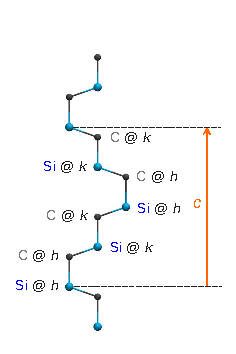
\includegraphics[width=0.38\textwidth]{figures/SiC-non-equiv-sites.pdf}%
        % B FIELD through current loop
\begin{tikzpicture}[scale=1.2, thick]
  \def\Rx{1.45}
  \def\Ry{0.43}
  \def\h{0.5}
  \def\H{3}
  \def\L{4}
  \def\NB{5}
  \def\ang{36}
  \coordinate (O) at (0,0);
  \coordinate (N) at (0,0.24*\H);
  \coordinate (M) at (0,0.45*\H);
  \coordinate (B) at (\ang:\H);
  
  % MAGNETIC FIELD
  \draw (-\Rx,0) arc (180:0:{\Rx} and {\Ry});
  \begin{scope}
    \clip ({-0.5*\L*cos(\ang)},-0.4*\H) rectangle ++({\L*cos(\ang)},\H);
    %\foreach \i [evaluate={\y=(\i-0.5)*\H/(\NB-0.5)/2;
    %                       \yl=-\H/2+(\i-0.5)*\H/(\NB-0.5)/2;}] in {1,...,\NB}{
    %  %\draw[BFieldLine,thin] (0,\y)++(\ang-180:0.5*\L) --++ (\ang:\L);
    %  %\draw[BFieldLine,thin] (0,-\y)++(\ang-180:0.5*\L) --++ (\ang:\L);
    %  \draw[BFieldLine,thin] (-\H/2,\y) -- ({-\H/2+(\H/2-\y)*cos(\ang)},\H/2);
    %  \draw[BFieldLine,thin] (-\H/2,-\y) -- ({-\H/2+(\H/2+\y)*cos(\ang)},+\H/2);
    %  \draw[BFieldLine,thin] ({\H/2-(\H/2+\yl)*cos(\ang)},-\H/2) -- (\H/2,\yl);
    %  \draw[BFieldLine,thin] ({\H/2-(\H/2-\yl)*cos(\ang)},-\H/2) -- (\H/2,-\yl);
    %}
    % \foreach \i [evaluate={\x=-0.31*\H+(\i-1)*0.62*\H/(\NB-1);
    %                        \y=-cot(\ang)*\x;
    %                        \a=0.50+0.017*\i}] in {1,...,\NB}{ %0.58-0.02*(\i-\NB/2-1)^2
    %   \draw[BFieldLine=\a] (\x,\y)++(\ang-180:\H) --++ (\ang:2*\H);
      %\fill[red] (\x,\y) circle (0.05);
    % }
  \end{scope}
  % \node[Bcol] at (\H/2,0.49*\H) {$\vb{B}$};
  
  % CIRCUIT
  \draw[white,very thick]
        (-\Rx,0) arc (-180:0:{\Rx} and {\Ry});
  \draw (-\Rx,0) arc (-180:0:{\Rx} and {\Ry});
  %\draw[white,very thick] (0,0) ellipse ({\R} and {0.3*\R});
  %\draw (0,0) ellipse ({\R} and {0.3*\R});
  %\draw (0,0) ellipse ({\R} and {0.3*\R});
  \draw[mu vector] (0,0) -- (M) node[above=-1, left=0] {$\vb*{\mu}$};
  \draw[vector] (0,0) -- (N) node[below=0,left=0] {$\vu{n}$};
  % \draw pic[->,"\small$\;\theta$",draw=black,angle radius=14,angle eccentricity=1.4]
    % {angle = B--O--N};
  \draw[white,very thick]
    (-150:{1.1*\Rx} and {1.16*\Ry}) arc (-150:-80:{1.1*\Rx} and {1.16*\Ry});
  \draw[current]
    (-135:{1.1*\Rx} and {1.16*\Ry}) arc (-135:-90:{1.1*\Rx} and {1.16*\Ry})
    node[midway,right=2,below] {$I$};
  
\end{tikzpicture}


  \caption{Schematic of current loop and induced magnetic moment.}%
\end{wrapfigure}%


The \index{magnetic dipole}{magnetic dipole} induces a magnetic field $\vec{B}$, which for points a large distance from the dipole may be calculated as \cite{Griffiths2012-pt}:
\begin{equation}
    \vec{B} = \frac{\mu_0}{4\pi} \frac{1}{r^3} \left[\frac{3(\vec{\mu} \cdot \vec{r}) \cdot \vec{r}}{r^2} - \vec{\mu}\right]
    \label{eq:}
\end{equation}

The symmetry of the field enables us to consider the direction of the dipole as aligned to the $z$-axis. Then, defining $x,y$ as usual by $r \cos\theta$ and $r \sin\theta$ respectively. We may decompose the \index{magnetic field}{magnetic field} in two separate components, parallel ($B_z$) and perpendicular ($B_x, B_y$): 
$$B_\parallel =\frac{\mu_0}{r^3}(3\cos^2 \theta - 1), \quad B_\perp = \frac{3\mu_0}{r^3}\cos\theta\sin\theta.$$
Where we use the Pythagorean principle to determine the overall magnitude $B = |\vec{B}|$ as
$$B = \sqrt{B_\parallel^2 + B_\perp^2}.$$

\input{Sections/RabiOscillations.tex}
\subsection{Gyromagnetic Ratio}
\subsubsection{Classical Derivation}
The current in equation \ref{eq:dipole_moment} is proportional to the angular momentum of the charge. That is, the dipole moment is always associated with an angular momentum $\vec{G} = \vec{r} \times \vec{p}$ with $\vec{r}$ the radius and $\vec{p}$ the momentum. 

Dividing the magnetic dipole moment by the angular momentum we find the \textbf{gyromagnetic ratio}. 
\begin{equation}
    \gamma = \frac{\vec{\mu}}{\vec{G}}.
    \label{eq:gyromagnetic_ratio}
\end{equation}

Without loss of generality we may consider the most simple case which is where the magnetic dipole moment is parallel (or anti-parallel) to the angular momentum. Then we may consider the absolute values for the dipole moment and the angular momentum: 
\begin{equation}
    \mu = IS, \quad I = 
    % \underbrace{\frac{q}{2\pi R}}_{\rho \text{ (charge density)}}v,
    \frac{qv}{2\pi R},
    \quad S = \pi R^2 
    % \label{eq:}
\end{equation}
We substitute $I$ and $S$ to find 
\begin{equation}
    \mu = \frac{qvR}{2} 
    % \label{eq:}
\end{equation}
% which we substitute into our equation for the gyromagnetic ratio 
% \begin{equation}
%     \gamma = \frac{\frac{qvR}{2}}{\vec{G}}. 
%     \label{eq:789}
% \end{equation}
and further, we equate the angular momentum vector, using the model of a planar loop to 
\begin{equation}
   G= m_q v R 
    % \label{eq:}
\end{equation}
leaving 
\begin{equation}
    \gamma = \frac{q}{2m_q } . 
    % \label{eq:}
\end{equation}

We finally consider that we may represent the, currently unknown, charge and mass as a sum of electron charges and masses. 
\begin{equation}
    \gamma = \frac{q}{2m_q } = \frac{\cancel{N}e}{2\cancel{N} m_e} \implies \gamma = \frac{e}{2 m_e}
    \label{eq:gyromagnetic_ratio}
\end{equation}

We therefore find that the gyromagnetic ratio of the electron depends only on fundamental constants \cite{bromley2000quantum}.

%pg 329 
% https://www.google.co.uk/books/edition/_/7qCMUfwoQcAC?hl=en&gbpv=1&bsq=walter%20greiner%20theoretical%20physics



\input{Sections/SpinInitialisation.tex}
\section{Lattice Symmetry}
Tetragonal lattice has the $$



\chapter{Task}
\section{Brief}

I think, as a start can go through section 3.2.4 in the attached PhD thesis? In particular check in details how to diagonalise the NV centre spin S=1 Hamiltonian to get Eq. 3.31?
You could also do some python simulations to plot how the spin levels (i.e. the eigenvalues of the spin Hamiltonian) change with applied magnetic field.

Once we've learned this, we can apply it to other spin defects in SiC.

\section{Work}
\subsection{Concepts and Nomenclature}
\subsubsection{Spin-Spin Interactions}
\subsubsection{Zeeman Splitting}
\subsubsection{Hyperfine Interaction}
\subsection{System Hamiltonian}\label{system_hamiltonian}
The ground state of the $\ce{NV^-}$ spin system in diamond is a triplet state, thus a $S=1$ system. 

The corresponding Hamiltonian, which it seems can be generalised to an electron spin system of a defect, can be expressed as: 
\begin{equation}
    H_{\ce{NV}} = H_{\ce{D}} + H_{\ce{Zeeman}} + H_{\ce{HF}} 
    \label{eq:nv_hamil}
\end{equation}

Here the labels $\ce{D}$, $\ce{Z}$ and $\ce{HF}$ describe the electron spin-spin interactions, the Zeeman interaction with an external magnetic field and the hyperfine interaction between the nuclparallel spin $I$ and the electron spin $S$ of the NV. 

They have the following forms: 
\begin{eqnarray}
    H_{\ce{D}} &=& D S_z^2 + E(S_x^2 + S_y^2) \label{H_D} \\
    H_{\ce{Z}} &=& g \mu_B \sum_{j}^{x,y,z} B_j \cdot S_j \label{H_Z} \\
    H_{\ce{HF}} &=& \vec{S} \cdot A \cdot \vec{I}. \label{H_HF}
\end{eqnarray}

\subsubsection{Spin-Spin Interaction}


The $E$ and $D$ in equation \ref{H_D} the fine structure constants of the spin
system, describing the spin-spin interaction and $S_j$ the corresponding spin operators
in x,y and z-direction. 

D is non-zero in system with axis of threefold (or other manifold) symmetry. 
The symmetry or spin quantization axis points along the connection of the nitrogen
atom and vacancy forming the defect. In bulk diamond $D$ is around 2.87 GHz at room temperature.

The definiteness, orientation and magnitude of $D$ is thus dependent on the specific spin system being studied. 

E occurs when there is a distortion of the point group symmetry, for example strain or an electrical field. In bulk diamond $E$ is typically negligibly small but especially in NDs, $E$ can be of the order of several MHz. 

Thus, similarly, the value of $E$ is a characteristic of the nature of the distortion and 
the specifics of the spin system being studied. 

\subsubsection{Zeeman Interaction}

$B_j$ in equation \ref{H_Z} is the magnetic field along the $x$, $y$ and $z$ direction, $g$ is the $g$-factor of the vacancy and $\mu_B$ the Bohr-Magneton, a constant. 

It seems often the scaled parameter $g\mu_B$ is considered, for the $\ce{NV^-}$ system this is around $28\;\ce{ GHz T^{-1}}$, but again, will be a characteristic of the system being studied. 

\subsubsection{Hyperfine Interaction}

Equation $\ref{H_HF}$ related the nuclear spin to the electron spin via the hyperfine tensor $A$ which has the form 
\begin{equation}
    A = \begin{pmatrix}
        A_\perp & 0 & 0 \\ 
        0 & A_\perp & 0 \\ 
        0 & 0 & A_\parallel
    \end{pmatrix}.
    \label{eq:hyperfine_tensor}
\end{equation}

$A_\parallel$ and $A_\perp$ are the axial and non-axial hyperfine parameters which encode two different interactions. 

\paragraph{Fermi Contact Interaction.}
This interaction is calculated by 
\begin{equation}
    f_A = \frac{A_\parallel + 2 A_\perp}{3}.
    \label{eq:fermi_contact}
\end{equation}

\paragraph{Anisotropic Interaction.}
This interaction is found by considering both spins as magnetic dipoles is calculated by 
\begin{equation}
    d_A = \frac{A_\parallel - A_\perp}{3}.
    \label{eq:anisotropic}
\end{equation}

For the $\ce{NV^-}$ system in diamond specifically, using the values for $A_\parallel$ and $A_\perp$ we calculate that $f_A$ is an order of magnitude stronger than $d_A$ for both $\ce{N^{14}}$ and $\ce{N^{15}}$. 

\subsubsection{Reduced Hamiltonian}
By combining $H_{\ce{D}}$ and $H_{\ce{Z}}$ 
and neglecting $H_{\ce{HF}}$ \todo{why (specifically) do we get to neglect this? Can we generalise?}
we find 
\begin{equation}
    H_{\ce{NV}} = D S_z^2 + E(S_x^2 + S_y^2) + g \mu_B \sum_{j}^{x,y,z} B_j \cdot S_j 
    \label{eq:reduced_H_NV}
\end{equation}

The spin operators $S_j$ in matrix representation are 
\begin{equation}
    S_x = \frac{1}{\sqrt{2}} \begin{pmatrix}
        0 & 1 & 0 \\ 
        1 & 0 & 1 \\ 
        0 & 1 & 0
    \end{pmatrix}, 
    S_y = \frac{i}{\sqrt{2}} \begin{pmatrix}
        0 & -1 & 0 \\ 
        1 & 0 & -1 \\ 
        0 & 1 & 0
    \end{pmatrix}, 
    S_z = \frac{1}{\sqrt{2}} \begin{pmatrix}
        1 & 0 & 0 \\ 
        0 & 0 & 0 \\ 
        0 & 0 & -1
    \end{pmatrix}. 
    \label{eq:spin_operators}
\end{equation}

Then, aligning the magnetic field (with strength $B_0$) along the $z$-axis (the quantisation axis), the reduced Hamiltonian will have the form 
\begin{equation}
    H_{\ce{NV}} = \begin{pmatrix}
        D + B_0 & 0 & E \\ 
        0 & 0 & 0 \\ 
        E & 0 & D-B_0
    \end{pmatrix},
    \label{eq:reduced_H_NV_matrix}
\end{equation}

with Eigenvalues 

\begin{equation}
    E_x = E_y = D \pm \sqrt{B_0^2  + E^2}, \; E_z = 0.
    \label{eq:reduced_H_NV_eigenvalues}
\end{equation}

The corresponding non-normalised Eigenvectors are then 

\begin{eqnarray}
    \ket{X} = \frac{1}{E} \left(B_0 + \sqrt{B_0^2 + E^2}\right) \ket{+1} + \ket{-1} \\ 
    \ket{Y} = \frac{1}{E} \left(B_0 - \sqrt{B_0^2 + E^2}\right) \ket{+1} + \ket{-1} \\ 
    \ket{Z} = \ket{0},
\end{eqnarray}
with
\begin{equation}
    \ket{1} = \begin{pmatrix}
        1 & 0 & 0 
    \end{pmatrix}, \; 
    \ket{0} = \begin{pmatrix}
        0 & 1 & 0 
    \end{pmatrix}\;, 
    \ket{-1} = \begin{pmatrix}
        0 & 0 & 1 
    \end{pmatrix},
    \label{eq:base_states}
\end{equation}
the Eigenvectors for $H_{\ce{NV}}$ with $E=0$\dots

In the case where $E \ll B_0$ the Eigenvectors are well described by the bases $\ket{0}$ and $\ket{\pm 1}$.

For $E \gg B_0$, when transforming the spin operators $S_j$ into the diagonalised system with Hamiltonian $H_{\ce{NV}}$ they read 
\begin{equation}
    \hat{S}_x^\parallel \propto \begin{pmatrix}
        0 & 1 & 0 \\ 
        1 & 0 & 0 \\ 
        0 & 0 & 0 
    \end{pmatrix} \; , 
    \hat{S}_y^\parallel \propto \begin{pmatrix}
        0 & 0 & 0 \\ 
        0 & 0 & -i \\ 
        0 & i & 0 
    \end{pmatrix} \; , 
    \hat{S}_z \propto \begin{pmatrix}
        0 & 0 & -1 \\ 
        0 & 0 & 0 \\ 
        -1 & 0 & 0 
    \end{pmatrix} , 
    \label{eq:diagonalised_spin_operators}
\end{equation}
and 
\begin{equation}
    \hat{H}_{\ce{NV}} = \begin{pmatrix}
        D + \sqrt{B_0^2 + E^2} & 0 & 0 \\ 
        0 & 0 & 0 \\ 
        0 & 0 & D - \sqrt{B_0^2 - E^2}. 
    \end{pmatrix} 
\end{equation}

Another solution for a $\pi/2$ shifted, modulating magnetic field leads to 
\begin{equation}
    \hat{S}_x^\perp \propto \begin{pmatrix}
        0 & 0 & 0 \\ 
        0 & 0 & 1 \\ 
        0 & 1 & 0 
    \end{pmatrix} \; , 
    \hat{S}_y^\perp \propto \begin{pmatrix}
        0 & -i & 0 \\ 
        i & 0 & 0 \\ 
        0 & 0 & 0 
    \end{pmatrix} \; , 
    \hat{S}_z \propto \begin{pmatrix}
        0 & 0 & 1 \\ 
        0 & 0 & 0 \\ 
        1 & 0 & 0 
    \end{pmatrix} , 
    \label{eq:diagonalised_spin_operators}
\end{equation}
a physical interpretation of which is that a linear modulating B-field aligned
along the $x$-axis where strain is applied only allows transitions between the state
$\ket{X}$ and $\ket{0}$, whereas fields perpendicular to the strain and the NV quantization axis
only allow coupling between $\ket{Y}$ and $\ket{0}$.

For an arbitrary external magnetic field, $H_\ce{NV}$ can be expressed using spherical co-ordinates: 
\begin{equation}
    H_{\ce{NV}} = \begin{pmatrix}
        D + B_0 \cdot \cos \theta & \frac{B_0}{\sqrt{2}} \cdot e^{-i\cdot \varphi} \cdot \sin\theta & E \\ 
        \frac{B_0}{\sqrt{2}} \cdot e^{i \cdot \varphi} \cdot \sin\theta & 0 & \frac{B_0}{\sqrt{2}} e^{-i\cdot \varphi} \cdot \sin\theta \\ 
        E & \frac{B_0}{\sqrt{2}} \cdot e^{i \cdot \varphi} \cdot \sin\theta & D - B_0 \cdot \cos \theta
    \end{pmatrix}
    \label{eq:nv_hamil_spherical_matrix}
\end{equation}


Here, we transformed the magnitude of the arbitrary magnetic field into spherical co-ordinates as 
\begin{eqnarray}
    B_x  &=& B_0 \cos\varphi \sin\theta \\ 
    B_y  &=& B_0 \sin\varphi \sin\theta \\ 
    B_z  &=& B_0 \cos\theta 
\end{eqnarray}
with $\theta$ the azimuthal and $\varphi$ the polar angle. Then using equations \ref{eq:reduced_H_NV} and \ref{eq:spin_operators} we compute \ref{eq:nv_hamil_spherical_matrix}.  

It immediately follows from the characteristic equation that Eigenvalues $\lambda$ satisfy 
\begin{equation}
    0 = \lambda^3 - 2\cdot \lambda^2 \cdot D + \frac{D \cdot B_0^2}{2} + \lambda(D^2 - E^2 - B_0^2) - \frac{1}{2}B_0^2\underbrace{\left(D \cdot \cos(2\theta) - 2 \cdot E \cos(2\varphi) \cdot \sin(\theta)^2\right)}_{\Delta_{\varphi \theta}}
    \label{eq:nv_spherical_characteristic_equation}
\end{equation}
% \cite{balasubramanian2009}





\chapter{Design}
%
% This section should be written in standard scientific
% language. Standard techniques in your research field should not be
% written out in detail. In computational projects this section should
% be used to explain the algorithms used and the layout of the
% computational code. A copy of the actual code may be given in the
% appendices if appropriate.
%
% This section should emphasise the philosophy of the approach used and
% detail novel techniques. However please note: this section should not
% be a blow-by-blow account of what you did throughout the project. It
% should not contain large detailed sections about things you tried and
% found to be completely wrong! However, if you find that a technique
% that was expected to work failed, that is a valid result and should be
% included.
%
% Here logical structure is particularly important, and you may find
% that to maintain good structure you may have to present the
% explorations/calculations/computations/whatever in a different order
% from the one in which you carried them out.
%
%
% You might sometimes want to include multiple equations in one place
% \begin{eqnarray}
%   E &=& ma^{2} \\
%   E &=& mb^{2} \\
%   E &=& mc^{2}
% \end{eqnarray}
% You might want to include multiple equations in one place without
% numbering them
% \begin{eqnarray*}
%   E &=& ma^{2} \\
%   E &=& mb^{2} \\
%   E &=& mc^{2}
% \end{eqnarray*}
% You might want to include multiple equations in one place without
% numbering \emph{all} of them
% \begin{eqnarray}
%   E &=& ma^{2} \nonumber \\
%   E &=& mb^{2} \nonumber \\
%   E &=& mc^{2}
% \end{eqnarray}
%
% You might also want to include diagrams.  The example shows the use of
% the special command which allows existing pdf files to be included.
% You would normally keep your figures separate from the text.  These
% pictures might be images or pdf output from some program.
%
% Here, I created a figure which is centred and stretched to 30\% of the
% width of the page \verb+{0.30\hsize}+ and with the height stretched by
% the same amount \verb+{!}+ to preserve the aspect ratio. If you omit
% the extension (ie .eps, .ps or .pdf) on the file name then \LaTeX\ will
% pick up the postscript copy whereas pdflatex will automatically pick
% up the PDF version.
%
%
% \begin{figure}
%
% \begin{center}
%   \resizebox{0.30\hsize}{!}{
\includegraphics{crest.pdf}}
% \end{center}
%
% \caption{The coloured version of the University crest. The caption should explain exactly in some detail what is displayed in the table.}
% \label{fig:eucrest}
%
% \end{figure}
%
% You should find the file crest.pdf on this wiki.
%
% % note that labels do not need to include a description of the object
% % they are labelling but it can be helpful, eg \label{fig:figurename}.
%
% You can use a label on a figure to refer to it later. The university
% crest is in Figure~(\ref{fig:eucrest}). Note that you should not use
% phrases like ``the figure above'' or ``the following figure'' since
% \LaTeX\ may move the figure relative to the text if it cannot be fitted
% onto the current page. The figure on the next page is an example.
%
%
%

\chapter{Results and Analysis}\label{ch:results}

Overall, the scope of multimodality which can be achieved depends very heavily on the complex interconnection of the parameter influence. Often, by constraining a freedom of one of the parameters the interplay is significantly simplified and allows for multimodal measurement. This is of course still relevant as many physical systems for which nanoscale sensors of this kind will be useful will have predictable characteristics. 

It has been shown in this work that by controlling other factors, defects in silicon carbide may be used as quantum sensors to detect both the electric and magnetic fields, pressure, strain and temperature. 

For multimodal sensing without constraint, the temperature independence of the ZFS $D$ parameter in the V2 Silicon vacancy showed the most obvious application. As briefly mentioned, further research into the interplay between temperature and any other characteristic will expand the scope of what it is possible to simultaneously sense. 

This allowed for sensing of magnetic field and temperature simultaneously - possibly even with the same defect family. With a long enough integration time, so assuming a steady state system, this measurement could potentially be made using only a single defect.

For constrained multimodal sensing, three more schemas were developed which exploit the reduction in complexity when the off diagonal terms in the Hamiltonian are reduced by precise field alignment. 

\todo[inline]{discuss each scheme 1 by 1, images?}

Without a developed schema for $\vec{E}$ field measurement with a $S=3/2$ system, the temperature stable ZFS $D$ was not able to be exploited and so we were not able to determine an unconstrained method for multimodal sensing involving the $\vec{E}$ field. 

An approach considered in this work, albeit unsuccessful was to attempt to reduce the ambiguity within some of the systems by comparing the effects on basal and c-axis defects. Similar schemes are used with the Diamond nitrogen vacancy, however that system has four distinct defect orientations and so integration into three dimensional space is overdetermined. Conversely for SiC there are only two distinct orientations and thus integration into three dimensional space is underdetermined. Further, at temperatures above cryogenic, some of the alternative defects produce very low contrast. Thus, in the context of multimodality, even if solved, the technique would likely be inappropriate. 


% \subsection{Successful}
% Here we discuss the proposed systems which could be successfully implemented using the techniques described in this work. 
% \subsubsection{$\vec{B}$ and Temperature}
% The fact that the V2 Silicon vacancy shows little to no correlation between the ZFS $D$ parameter and temperature makes it 
% extremely useful for multimodal sensing. The ODMR spectra of the  defect is effectively blind to temperature allowing it to be 
% paired with another defect (or technique) very easily. 
%
% \missingifigure{Plot showing ODMR simulated spectra at $B$ constant, $T$ varied (showing no difference). }
%
% The fact that the anti-Stokes measurement of temperature depends strongly on the position of the zero phonon line, which is determined by $D$ allows for the use of a single defect type to measure both parameters. This single defect dependence allowed for the discussion of tri-modal sensing which is discussed at the end of this chapter. 
%
% Further, the stability of the $D$ parameter is what enables the anti-Stokes method to be employed (and hinders other systems). 
% The method relies on using two lasers of wavelengths strictly larger and smaller than the zero phonon line. If $D$ was varying, laser frequencies would have to be adjusted on the fly, may be technically possible, but limits the utility of the system. 
%
% \subsubsection{$\vec{B}$, Temperature and $\vec{E}$}
% A tri-modal system 
%
% \subsection{Not Successful}
%
% \subsection{High Potential}
% The obvious high potential multimodal system is a temperature pressure measurement. 
% The applications of such a sensor are obvious and immediate.  
% The consistency of the ZFS $D$ parameter in the V2 Silicon vacancy, but strong dependence on pressure .



%%%%%%%%%%% CLEAR presentation of results presented graphically where possible 
% \lipsum[1-2]
% \missingfigure{Add a figure to illustrate}
%
% \lipsum[1-2]
% \missingfigure{Add a figure to illustrate}
%
% \lipsum[1-2]
% \missingfigure{Add a figure to illustrate}
%
% \lipsum[1-2]
% \missingfigure{Add a figure to illustrate}
%
% This section should detail the obtained results in a clear,
% easy-to-follow manner. It is important to make clear what are original
% results and what are repeats of previous calculations or computations.
% Remember that long tables of numbers are just as boring to read as
% they are to type-in!
%
% Use graphs to present your results wherever practicable.
%
% Results or computations should be presented with uncertainties
% (errors), both statistical and systematic where applicable.
%
% Be selective in what you include: half a dozen \emph{e.g.}~tables that
% contain wrong data you collected while you forgot to switch on the
% computer are not relevant and may mask the correct results.
%
%
% \section{Some results}
% Here are some results.
%
% \subsection{More results}
% When showing results you are likely to use tables and graphs. You can
% create tables easily in \LaTeX.
%
% \begin{table}[h]
% \begin{center}
% \begin{tabular}{||l|c|l||}
% \hline
% \textbf{File names} & \textbf{Satellite} & \textbf{Resolution}\\
% \hline
%   worldr            &  Meteosat          &   5km\\
%   worldg            &  Meteosat          &   5km\\
%   worldb            &  Meteosat          &   5km\\
% \hline
% \end{tabular}
% \end{center}
% \caption{This is a simple table. More complicated tables can have
%   headings which pass over more than one column. The caption should
%   explain exactly in some detail what is displayed in the table.}
% \label{simple_table}
% \end{table}
%
% If you want to produce fancier tables than shown in Table \ref{simple_table}
% refer to the \LaTeX\ manual or ask Madame La Google.
%
% One of the simplest ways to produce simple graphs is to use gnuplot
% which produces \LaTeX\  output. Graph~(\ref{fig:gnu}) was produced using
% gnuplot with output designated as \LaTeX\  so that a \LaTeX\  output file is
% produced which you can include directly or keep separate and refer to
% using the \emph{include} command.
%
% Another approach is to draw simple figures using \emph{xfig} which allows
% you to export diagrams in \LaTeX\  picture format so that the diagram can
% be included directly.
%
% Perhaps the most robust way to include graphs is to convert them to
% PostScript or PDF and include them in the same was as was done in
% Figure~\ref{fig:eucrest} for the University Crest. You can usually do
% this with most packages, including Microsoft ones; one trick for
% producing PostScript is to print to a dummy PostScript printer.
%
% % in practice you would probably keep this in a separate file and use
% % the \include{filename} command to insert it here.
%
% \begin{figure}
% % GNUPLOT: LaTeX picture
% \setlength{\unitlength}{0.240900pt}
% \ifx\plotpoint\undefined\newsavebox{\plotpoint}\fi
% \sbox{\plotpoint}{\rule[-0.200pt]{0.400pt}{0.400pt}}%
% \begin{picture}(1500,1200)(0,0)
% \font\gnuplot=cmr10 at 10pt
% \gnuplot
% \sbox{\plotpoint}{\rule[-0.200pt]{0.400pt}{0.400pt}}%
% \put(220.0,113.0){\rule[-0.200pt]{292.934pt}{0.400pt}}
% \put(220.0,113.0){\rule[-0.200pt]{0.400pt}{245.477pt}}
% \put(220.0,113.0){\rule[-0.200pt]{4.818pt}{0.400pt}}
% \put(198,113){\makebox(0,0)[r]{$0$}}
% \put(1416.0,113.0){\rule[-0.200pt]{4.818pt}{0.400pt}}
% \put(220.0,317.0){\rule[-0.200pt]{4.818pt}{0.400pt}}
% \put(198,317){\makebox(0,0)[r]{$0.2$}}
% \put(1416.0,317.0){\rule[-0.200pt]{4.818pt}{0.400pt}}
% \put(220.0,521.0){\rule[-0.200pt]{4.818pt}{0.400pt}}
% \put(198,521){\makebox(0,0)[r]{$0.4$}}
% \put(1416.0,521.0){\rule[-0.200pt]{4.818pt}{0.400pt}}
% \put(220.0,724.0){\rule[-0.200pt]{4.818pt}{0.400pt}}
% \put(198,724){\makebox(0,0)[r]{$0.6$}}
% \put(1416.0,724.0){\rule[-0.200pt]{4.818pt}{0.400pt}}
% \put(220.0,928.0){\rule[-0.200pt]{4.818pt}{0.400pt}}
% \put(198,928){\makebox(0,0)[r]{$0.8$}}
% \put(1416.0,928.0){\rule[-0.200pt]{4.818pt}{0.400pt}}
% \put(220.0,1132.0){\rule[-0.200pt]{4.818pt}{0.400pt}}
% \put(198,1132){\makebox(0,0)[r]{$1$}}
% \put(1416.0,1132.0){\rule[-0.200pt]{4.818pt}{0.400pt}}
% \put(220.0,113.0){\rule[-0.200pt]{0.400pt}{4.818pt}}
% \put(220,68){\makebox(0,0){$0$}}
% \put(220.0,1112.0){\rule[-0.200pt]{0.400pt}{4.818pt}}
% \put(414.0,113.0){\rule[-0.200pt]{0.400pt}{4.818pt}}
% \put(414,68){\makebox(0,0){$1$}}
% \put(414.0,1112.0){\rule[-0.200pt]{0.400pt}{4.818pt}}
% \put(607.0,113.0){\rule[-0.200pt]{0.400pt}{4.818pt}}
% \put(607,68){\makebox(0,0){$2$}}
% \put(607.0,1112.0){\rule[-0.200pt]{0.400pt}{4.818pt}}
% \put(801.0,113.0){\rule[-0.200pt]{0.400pt}{4.818pt}}
% \put(801,68){\makebox(0,0){$3$}}
% \put(801.0,1112.0){\rule[-0.200pt]{0.400pt}{4.818pt}}
% \put(995.0,113.0){\rule[-0.200pt]{0.400pt}{4.818pt}}
% \put(995,68){\makebox(0,0){$4$}}
% \put(995.0,1112.0){\rule[-0.200pt]{0.400pt}{4.818pt}}
% \put(1188.0,113.0){\rule[-0.200pt]{0.400pt}{4.818pt}}
% \put(1188,68){\makebox(0,0){$5$}}
% \put(1188.0,1112.0){\rule[-0.200pt]{0.400pt}{4.818pt}}
% \put(1382.0,113.0){\rule[-0.200pt]{0.400pt}{4.818pt}}
% \put(1382,68){\makebox(0,0){$6$}}
% \put(1382.0,1112.0){\rule[-0.200pt]{0.400pt}{4.818pt}}
% \put(220.0,113.0){\rule[-0.200pt]{292.934pt}{0.400pt}}
% \put(1436.0,113.0){\rule[-0.200pt]{0.400pt}{245.477pt}}
% \put(220.0,1132.0){\rule[-0.200pt]{292.934pt}{0.400pt}}
% \put(45,622){\makebox(0,0){\shortstack{This is\\the\\$y$ axis}}}
% \put(828,23){\makebox(0,0){This is the $x$ axis}}
% \put(828,1177){\makebox(0,0){This is a plot of $y=\sin(x)$}}
% \put(220.0,113.0){\rule[-0.200pt]{0.400pt}{245.477pt}}
% \sbox{\plotpoint}{\rule[-0.500pt]{1.000pt}{1.000pt}}%
% \put(1306,1067){\makebox(0,0)[r]{sin(x)}}
% \multiput(1328,1067)(20.756,0.000){4}{\usebox{\plotpoint}}
% \put(1394,1067){\usebox{\plotpoint}}
% \put(220,113){\usebox{\plotpoint}}
% \multiput(220,113)(3.768,20.411){4}{\usebox{\plotpoint}}
% \multiput(232,178)(4.132,20.340){3}{\usebox{\plotpoint}}
% \multiput(245,242)(3.825,20.400){3}{\usebox{\plotpoint}}
% \multiput(257,306)(3.884,20.389){3}{\usebox{\plotpoint}}
% \multiput(269,369)(3.944,20.377){3}{\usebox{\plotpoint}}
% \multiput(281,431)(4.326,20.300){3}{\usebox{\plotpoint}}
% \multiput(294,492)(4.137,20.339){3}{\usebox{\plotpoint}}
% \multiput(306,551)(4.276,20.310){3}{\usebox{\plotpoint}}
% \multiput(318,608)(4.693,20.218){3}{\usebox{\plotpoint}}
% \multiput(331,664)(4.583,20.243){2}{\usebox{\plotpoint}}
% \multiput(343,717)(4.754,20.204){3}{\usebox{\plotpoint}}
% \multiput(355,768)(5.034,20.136){2}{\usebox{\plotpoint}}
% \multiput(367,816)(5.760,19.940){2}{\usebox{\plotpoint}}
% \multiput(380,861)(5.579,19.992){3}{\usebox{\plotpoint}}
% \put(398.00,923.50){\usebox{\plotpoint}}
% \multiput(404,943)(7.049,19.522){2}{\usebox{\plotpoint}}
% \multiput(417,979)(7.288,19.434){2}{\usebox{\plotpoint}}
% \put(433.18,1021.10){\usebox{\plotpoint}}
% \multiput(441,1040)(8.982,18.712){2}{\usebox{\plotpoint}}
% \put(460.41,1076.97){\usebox{\plotpoint}}
% \put(471.84,1094.28){\usebox{\plotpoint}}
% \put(484.84,1110.41){\usebox{\plotpoint}}
% \put(500.42,1124.01){\usebox{\plotpoint}}
% \multiput(503,1126)(19.159,7.983){0}{\usebox{\plotpoint}}
% \put(519.48,1131.37){\usebox{\plotpoint}}
% \multiput(527,1132)(20.136,-5.034){0}{\usebox{\plotpoint}}
% \put(539.74,1128.60){\usebox{\plotpoint}}
% \put(557.04,1117.38){\usebox{\plotpoint}}
% \put(570.79,1101.95){\usebox{\plotpoint}}
% \put(582.44,1084.80){\usebox{\plotpoint}}
% \put(593.09,1066.99){\usebox{\plotpoint}}
% \multiput(601,1053)(8.430,-18.967){2}{\usebox{\plotpoint}}
% \put(619.18,1010.54){\usebox{\plotpoint}}
% \multiput(625,996)(7.413,-19.387){2}{\usebox{\plotpoint}}
% \multiput(638,962)(6.403,-19.743){2}{\usebox{\plotpoint}}
% \multiput(650,925)(5.830,-19.920){2}{\usebox{\plotpoint}}
% \multiput(662,884)(5.461,-20.024){2}{\usebox{\plotpoint}}
% \multiput(674,840)(5.533,-20.004){2}{\usebox{\plotpoint}}
% \multiput(687,793)(4.937,-20.160){3}{\usebox{\plotpoint}}
% \multiput(699,744)(4.667,-20.224){2}{\usebox{\plotpoint}}
% \multiput(711,692)(4.858,-20.179){3}{\usebox{\plotpoint}}
% \multiput(724,638)(4.276,-20.310){3}{\usebox{\plotpoint}}
% \multiput(736,581)(4.205,-20.325){3}{\usebox{\plotpoint}}
% \multiput(748,523)(4.070,-20.352){3}{\usebox{\plotpoint}}
% \multiput(760,463)(4.326,-20.300){3}{\usebox{\plotpoint}}
% \multiput(773,402)(3.884,-20.389){3}{\usebox{\plotpoint}}
% \multiput(785,339)(3.884,-20.389){3}{\usebox{\plotpoint}}
% \multiput(797,276)(4.070,-20.352){3}{\usebox{\plotpoint}}
% \multiput(810,211)(3.825,-20.400){3}{\usebox{\plotpoint}}
% \multiput(822,147)(3.607,-20.440){2}{\usebox{\plotpoint}}
% \put(828,113){\usebox{\plotpoint}}
% \end{picture}
% \caption{Simple Gnuplot example. The caption should tell the reader
%   what is plotted against what, and explain in some detail the various
%   sets of curves of data points. It shouldn't just say ``plot of
%   results for the purple function in green gauge'' without further explanation.}
% \label{fig:gnu}
% \end{figure}
%
% \section{Discussion of your results}
%
% This section should give a picture of what you have taken out of your
% project and how you can put it into context.
%
% This section should summarise the results obtained, detail conclusions
% reached, suggest future work, and changes that you would make if you
% repeated the project.
%
%

\chapter{Conclusions}\label{ch:conclusions}
%%%%%%%%%%%%%%%%%%%%%%%%%%%%%%%%%%%% 1-2 Pages %%%%%%%%%%%%%%%%%%%%%%%%%%%%

% \lipsum[1]
\section{Multimodal Spin Based Sensors}
% \lipsum[2-4]
\section{Wider Scientific Context}
% The analysis based on the experimentally obtained parameters shows that this property can be used to implement solid-state masers and extraordinarily sensitive radiofrequency amplifiers.
\cite{Kraus2013}
% \lipsum[5-8]

\section{Future Work}
% \lipsum[9]
%
% This is the place to put your conclusions about your work. You can
% split it into different sections if appropriate. You may want to include
% a section of future work which could be carried out to continue your
% research.
%
% The conclusion section should be at least one page long, preferably 2
% pages, but not much longer.
%
%





% the appendix command just changes heading styles for appendices.
\appendix

% \chapter{Stuff that's too detailed}

Appendices should contain all the material which is considered too
detailed to be included in the main body of the text, but which is
important enough to be included in the thesis.

Perhaps this is a good place to mention \BibTeX.

You can do references in the simple way explained in the introduction,
or you can use \BibTeX.


\section{\BibTeX}
\label{sec:bibtex}

It is convenient to use \BibTeX\ to compile your bibliography.  First
you need to create a .bib file e.g.  you may call it ref.bib Then you
can put all your references into the file with entries such as
\begin{verbatim}
@Book{ob:bornwolf,
     author = "Born, M and Wolf, E",
     title  = "Principles of Optics",
     publisher = "Cambridge University Press",
     year = 1999,
     edition = {7th},
}

@Article{jr:ashkin,
Author = {A. Ashkin and J.M. Dziedzic and J.E. Bjorkholm and S. Chu},
Title = "Observation of a single beam gradient force optical tap for 
dielectric particles",
Journal = "Optics Letters",
Volume = 11,
Pages = "288-290",
Year = 1986}

@INPROCEEDINGS{seger,
 author = {J. Seger and H.J. Brockman},
 title = {What is bet-hedging?},
 editors={P.H. Harvey and L. Partridge},
 booktitle = {Oxford Surveys in Evolutionary Biology},
 year={1987},
 page={18},
 publisher={Oxford University Press},
 place={Oxford}}
\end{verbatim}
for a book, an article in a journal or an article in a proceedings volume
respectively.

Inside your \LaTeX\ file
you should include 
\begin{verbatim}
\bibliographystyle{unsrt}                      
and
\bibliography{ref}
\end{verbatim}
The first command determines the reference style, here plain and 
unsorted. With this referencing style 
a numerical referencing system (which is now the most
common in physics literature) is used and the numbering of references
will be the order in which they appear in the document. Alternatively, 
you could use
a customised `style file' but there is no real need.  The second
command just inputs your .bib file Note that only the references cited
in the text will appear in the bibliography so you can have spare
references in your .bib file.


You use the name you have given to an entry (e.g.
for the book example above the name is ob:bornwolf)
to cite the relevant article
by using the cite command in your \LaTeX\ file e.g. 
\begin{verbatim}
\cite{ob:bornwolf}
\end{verbatim}


\section{Producing your documents using \texttt{pdflatex}}

To use pdflatex your figures need to be in pdf format.  You can convert almost any image file to pdf using \texttt{convert}.  e.g. \texttt{convert myfigure.png myfigure.pdf}.

The first time you should type:
\begin{verbatim}
  pdflatex ProjectReport
  bibtex ProjectReport
  pdflatex ProjectReport
  pdflatex ProjectReport
\end{verbatim} 
This first time you run\texttt{pdflatex} it will produce a
\texttt{ProjectReport.aux}.  The \BibTeX\ command reads in the
bibliography file and makes the files \texttt{ProjectReport.bbl} and
\texttt{ProjectReport.blg} files.  These files are read in the next
\texttt{pdflatex} command, but you'll still have ``undefined
cross-reference'' errors which are sorted out by the last
\texttt{pdflatex} command.

Subsequently, you should only need to do one (or two)
\texttt{pdflatex}s, or \texttt{pdfbibtex} followed by
\texttt{pdflatex} twice if you change any references.

\vspace{5mm} You may also use plain \texttt{latex} instead of
\texttt{pdflatex}.  This requires you to use postscript graphics
instead of pdf.






% \chapter{Stuff that won't be read by anyone}


Some people include in their thesis a lot of detail, particularly lots
of tables containing raw results, figures of intermediate results, or
computer code which no-one will ever read. You should be careful that
anything like this you include should contain some element of
uniqueness which justifies its inclusion.



% \chapter{Python Code}

This project utilised a model of the electron systems which was built using Python. Source code can be found at \url{https://www.github.com/cadlinga}. 
% \lstinputlisting[language=Python, size=small, title={`main.py'}]{python/main.py}

\nocite{*}
\printindex
\bibliography{ref}

\end{document}

